\documentclass[a4paper, twoside]{report}

%pacchetti da laboratorio
\usepackage[utf8]{inputenc} % lettere accentate da tastiera
\usepackage[italian]{babel} % lingua del documento
\usepackage{amsmath}        %serve per scrivere un testo negli array
\usepackage{amssymb}
\usepackage{booktabs}       %migliora le linee delle tabelle
\usepackage{fancyhdr}       %permette di modificare l' intestazione della pagina
\usepackage{float}
\usepackage{moreverb}
\usepackage{ifthenx}
\usepackage{graphicx}
\usepackage{caption}
\usepackage{placeins}
\usepackage{eepic,epic,eepicemu}
\usepackage{color}
\usepackage{bm}  %messo da me per grassetto in $$
\usepackage{caption} %messo da me per caption in minipage

%pacchetti da tesi inlgese
%\usepackage[utf8x]{inputenc} 
\usepackage[T1]{fontenc}
\usepackage{listings}
\usepackage{hyperref}
\hypersetup{colorlinks=false}
\usepackage{lscape}
\usepackage{subfigure}
\usepackage{amsmath}
\usepackage{graphicx}
\usepackage[colorinlistoftodos]{todonotes}
\usepackage[a4paper,top=3cm,bottom=2cm,left=3cm,right=3cm,marginparwidth=1.75cm]{geometry}


\title{Studio della produzione del mesone $D^{*+}$ con metodi multivariati}
\author{Laura Pintucci}
% Update supervisor and other title stuff in title/title.tex

\begin{document}

%_________________PAGINA TITOLO_______________________________
\begin{titlepage}

\newcommand{\HRule}{\rule{\linewidth}{0.5mm}} % Defines a new command for the horizontal lines, change thickness here

%\begin{multicols}{hnumeroi}
%htesto multicolonnai
%\end{multicols}



%----------------------------------------------------------------
%	LOGO SECTION
%----------------------------------------------------------------
\noindent
\begin{minipage}{.32\textwidth} %{0.5 cm}
\begin{flushleft} \large
\flushleft
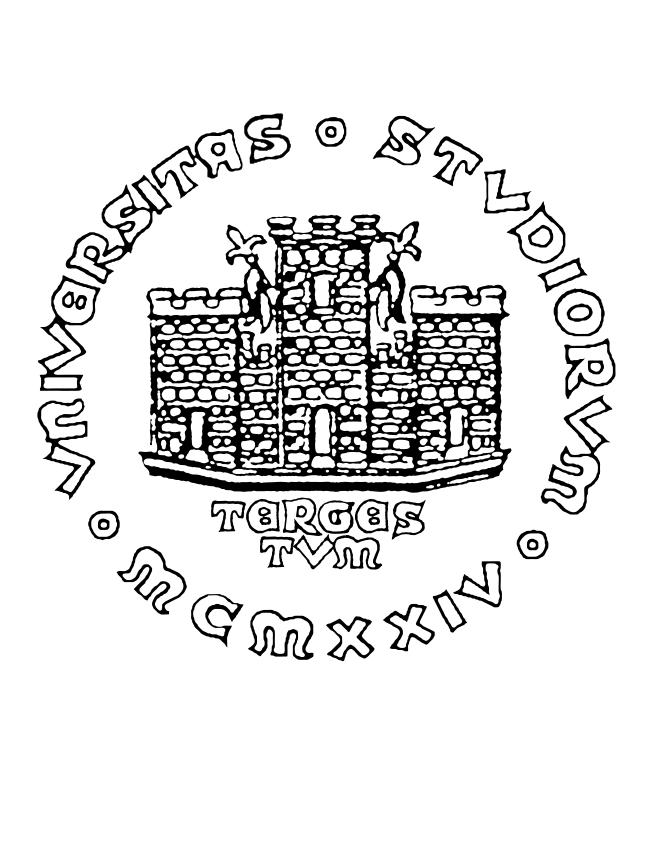
\includegraphics[width=4cm]{title/sigilloUniTS.png}
\end{flushleft}
\end{minipage}
~
\begin{minipage}{0.65\textwidth}
\begin{flushright} \large
\textsc{\normalsize Università degli Studi di Trieste}\\[0.2cm] 
\textsc{\normalsize Dipartimento di Fisica }\\[0.4cm]
%{\large Dipartimento di Fisica}\\[0.5cm]
{\normalsize Corso di Laurea Triennale in Fisica}\\[0.3cm]

\end{flushright}
\end{minipage}\\[1cm]
\makeatother


%----------------------------------------------------------------
\center % Center everything on the page

%----------------------------------------------------------------
%	HEADING SECTIONS
%----------------------------------------------------------------
\quad\\[1.5cm]
{\normalsize Tesi di Laurea Triennale}\\[0.5cm]
%\textsc{\LARGE MSc Thesis}\\[1.5cm] % Name of your university/college
%\textsc{\Large Università degli Studi di Trieste}\\[0.5cm] % Major heading s

%----------------------------------------------------------------
%	TITLE SECTION
%----------------------------------------------------------------
\makeatletter
\HRule \\[0.4cm]
{ \huge \bfseries \@title}\\[0.4cm] % Title of your document
\HRule \\[2.5cm]
 
%----------------------------------------------------------------
%	AUTHOR SECTION
%----------------------------------------------------------------

\begin{minipage}{0.4\textwidth}
\begin{flushleft} \large
\emph{Laureando:}\\
\@author % Your name
\end{flushleft}
\end{minipage}
~
\begin{minipage}{0.4\textwidth}
\begin{flushright} \large
\emph{Relatore:} \\
RU Grazia Luparello
\\[1.2em] % Supervisor's Name
\emph{Correlaotre:} \\
Prof. Paolo Camerini % second marker's name
\end{flushright}
\end{minipage}\\[5cm]
\makeatother


%----------------------------------------------------------------------------------------
%	DATE SECTION
%----------------------------------------------------------------------------------------

{\large Anno Accademico 2018/2019 }\\[0.5cm]
%{\large \today}\\[2cm] % Date, change the \today to a set date if you want to be precise

\vfill % Fill the rest of the page with whitespace

\end{titlepage}
\thispagestyle{empty} 
https://it.overleaf.com/project/5d4947035cf196734f993729
\cleardoublepage
https://it.overleaf.com/project/5d4947035cf196734f993729
%\renewcommand{\abstractname}{Acknowledgements}
%\begin{abstract}
%It is usual to thank those individuals who have provided %particularly useful assistance, technical or otherwise, during %your project.
%\end{abstract}


%________________PAGINA CITAZIONE_____________________________
\thispagestyle{empty} 
\begin{flushright}%{0.65\textwidth}
\null \vspace {\stretch {1}}

CITAZIONE DA TROVARE

\vspace {\stretch {2}}\null
\end{flushright}





%_________________PAGINA ABSTRACT______________________________
\begin{abstract}
SCRIVERE IL SOMMARIO
\end{abstract}

%________________SOMMARI_______________________________________

\tableofcontents
\listoffigures
\listoftables
Commenti generali: 
\chapter{Introduzione}

L'obbiettivo di questa tesi è quello di studiare la produzione del mesone $D^{*+}$ in collisioni protone protone generate ad LHC (Large Hadrons Collider), utilizzando i dati dell'esperimento ALICE (A Large Ion Collider Experiment). Lo studio della produzione del mesone $D^{*+}$ in questa tesi verrà condotto con metodi di analisi multivariata e in particolare utilizzando un Boosted Decision Tree (BDT). I dati che si utilizzeranno per l'analisi sono stati raccolti da ALICE nel 2017, sono caratterizzati da un'energia nel centro di massa di 5 $TeV$ e sono relativi a 985 milioni di collisioni. Alla fine del lavoro di questa tesi si vogliono confrontare i risultati ottenuti con il Boosted Decision Tree con quelli dell'analisi standard svolta ad ALICE.
\\Lo studio di mesoni con charm come il mesone $D^{*+}$, prodotti da collisioni di ioni pesanti ad ALICE, è importante per ottenere informazioni sul Quark Gluon Plasma (QGP). Questo è uno stato della materia che si formerebbe circa un picosecondo dopo la collisione tra i fasci di ioni, secondo la teoria della Cromo-Dinamica Quantistica (QCD).
In questa tesi si sono studiati i mesoni $D^{*+}$ prodotti da collisione di fasci di protoni, da cui non si forma il QGP. Questi dati vengono confrontati con quelli relativi a mesoni con charm prodotti da collisioni di ioni pesanti e che quindi hanno interagito con il QGP.
\\In questa tesi si vogliono selezionare le tracce relative al mesone $<D^{*+}$ tra tutte le tracce raccolte da ALICE. Questo è un tipico problema di selezione, in cui si cerca un segnale raro in un insieme di dati composto principalmente da eventi di fondo. L'utilizzo di algoritmi di machine learning come il BDT può essere utile per risolvere problemi di selezione. Per l'analisi dati svolta nel seguente lavoro di tesi si utilizza il TMVA (Tool for MultiVariate Analysis), uno strumento di Root, il quale permette di utilizzare algoritmi di analisi multivariata, tra cui il BDT. L'utilizzo del Boosted Decision Tree prevede due fasi principali. La prima è la fase di training, che viene svolta per far apprendere all'algoritmo le caratteristiche dei dati del segnale utilizzando dati di cui si conosce già la separazione tra segnale e fondo. In questa tesi si utilizzeranno per la fase di training dati ottenuti da simulazione Monte Carlo. La seconda fase è l'applicazione, in cui il BDT analizza i dati e li separa tra segnale e fondo, in base a quanto ha appreso durante la fase di training.
\\L'obbiettivo ultimo di questa tesi è calcolare quanti mesoni $D^{*+}$ sono stati selezionati con l'analisi del BDT e confrontare questi valori con quelli relativi all'analisi standard di ALICE. In questo modo si potrà valutare l'utilità di algoritmi di analisi multivariata per l'analisi dati di problemi di selezione ad ALICE.
\\Il contenuto del lavoro di questa tesi è strutturato come segue:
    \begin{itemize}
        \item CAPITOLO 2: breve introduzione sull'esperimento ALICE e i suoi rivelatori, da cui sono stati raccolti i dati che verranno utilizzati in questa tesi;
        \item CAPITOLO 3: breve introduzione sulla fisica particellare e sul mesone $D^{*+}$ studiato in questa tesi;
        \item CAPITOLO 4: breve introduzione agli algoritmi di analisi multivariati e al funzionamento del Boosted Decision Tree;
        \item CAPITOLO 5: descrizione della fase di training del BDT e dei risultati ottenuti;
        \item CAPITOLO 6: descrizione dell'applicazione del BDT sui dati di ALICE e valutazione dell'analisi svolta.
    \end{itemize}

\chapter{ALICE ad LHC}

\section{LHC}
A poca distanza da Ginevra si trova il più grande collisore di particelle del mondo: il \textit{Large Hadron Collider} (LHC). Questo acceleratore ha un raggio complessivo di 27~Km ed è stato costruito a partire dal 1998 dall'Organizzazione Europea per la Ricerca Nucleare (Cern) con lo scopo di progredire nella conoscenza dell'Universo e dei suoi meccanismi più profondi.
\\In figura \ref{fig:CERNcomplex} è mostrato il complesso di acceleratori del CERN, di cui LHC rappresenta l'ultimo stadio. L'insieme degli acceleratori \`e composto da un iniziale acceleratore lineare (Linac2), seguono tre sincrotroni, il Proton Synchrotron Booster (PSB), il Proton Synchrotron (PS) e il Super Proton Synchrotron (SPS), dal quale si ottengono particelle accelerate a 450~GeV, che vengono infine iniettate nell'LHC dove raggiungono un'energia di 6.5~TeV. 
 
    \begin{figure}[htbp]
        \centering
        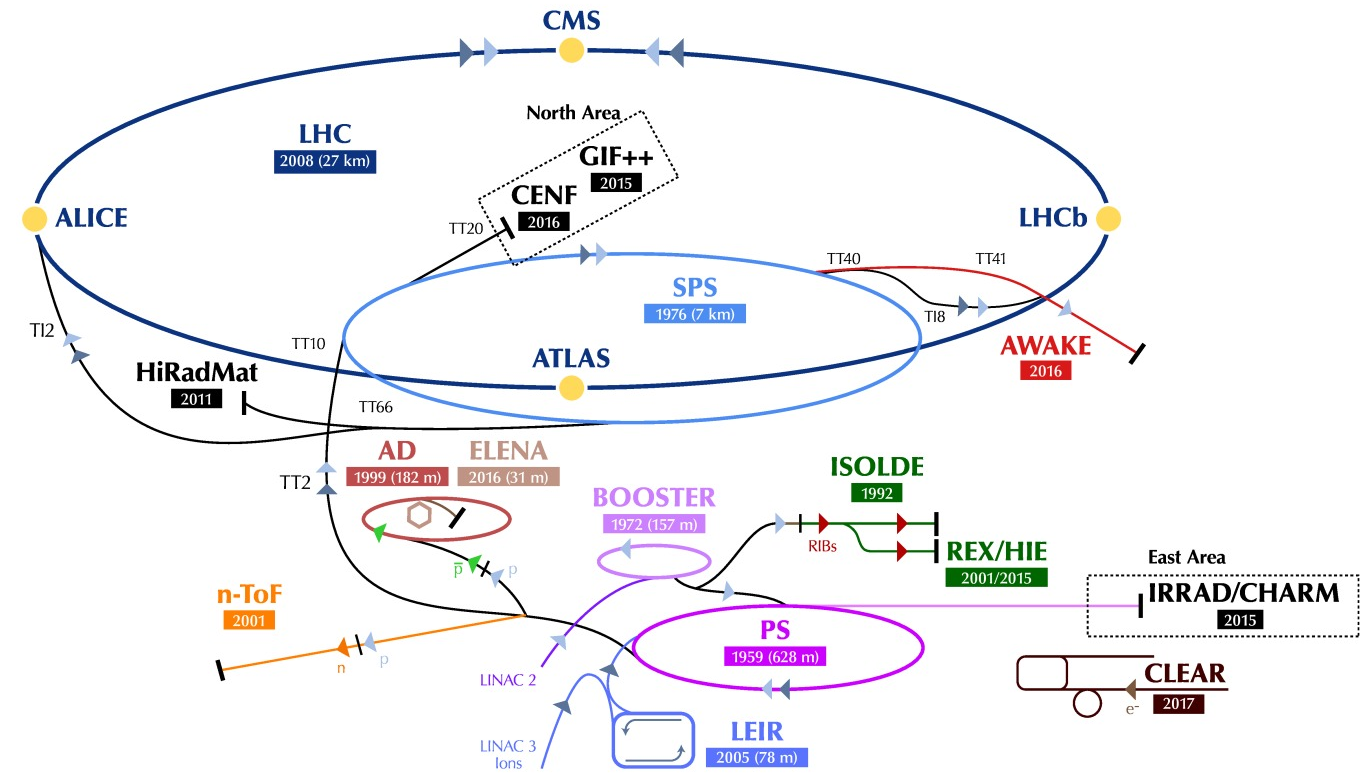
\includegraphics[width=0.8\linewidth]{ALICE/CernComplex_2018.png}   
        \caption{Complesso dell'intero acceleratore del CERN \\\small{Si vedono  \textcolor{blue}{LHC \textit{Large Hadron Collider}} \textcolor{cyan}{SPS \textit{Super Proton Synchrotron}} \textcolor{purple}{ PS \textit{Proton Synchrotron}} \textcolor{violet}{BOOSTER \textit{Proton Synchrotron Booster}} LINAC \textit{Linear ACcelerator}} \\{\footnotesize  \textcolor{red}{AD \textit{Antiprotron Decelerator}} \textcolor{green}{ISOLDE \textit{Isotope Separator Online DEvice}}  \textcolor{lightgray}{LEIR \textit{Low Energy Ion Ring}} }}
        \label{fig:CERNcomplex}
    \end{figure}
    
Il fascio di particelle viaggia in un tubo in cui viene fatto l'ultra-vuoto ed è direzionato da dei magneti superconduttivi tenuti alla temperatura di 1.85~K.

\section{ALICE}

L'acronimo ALICE sta per \textit{"A Large Ion Collider Experiment"} e lo  scopo primario dell'esperimento è quello di studiare la materia nucleare ad alte densità e alte temperature in uno stato chiamato \textit{Plasma di Quark e Gluoni} (QGP). Il QGP è caratterizzato da quark e gluoni liberi e non confinati negli adroni dalla forza nucleare forte. ALICE è ottimizzato per lo studio delle collisioni ad energie ultra-relativistiche di ioni pesanti (come il Piombo) in cui si raggiungono le condizioni necessarie per la formazione del QGP. Lo studio del QGP permette di comprendere le proprietà di questo stato della materia, la cui esistenza è prevista dalla Cromo-Dinamica Quantistica, e di comprendere come si sia formata la materia ordinaria, dal momento che si suppone che fino a $10^{-6}$ s dopo il Big-Bang la materia esistesse solo nello stato di QGP.  
    
    \begin{figure}[htbp]
        \centering
        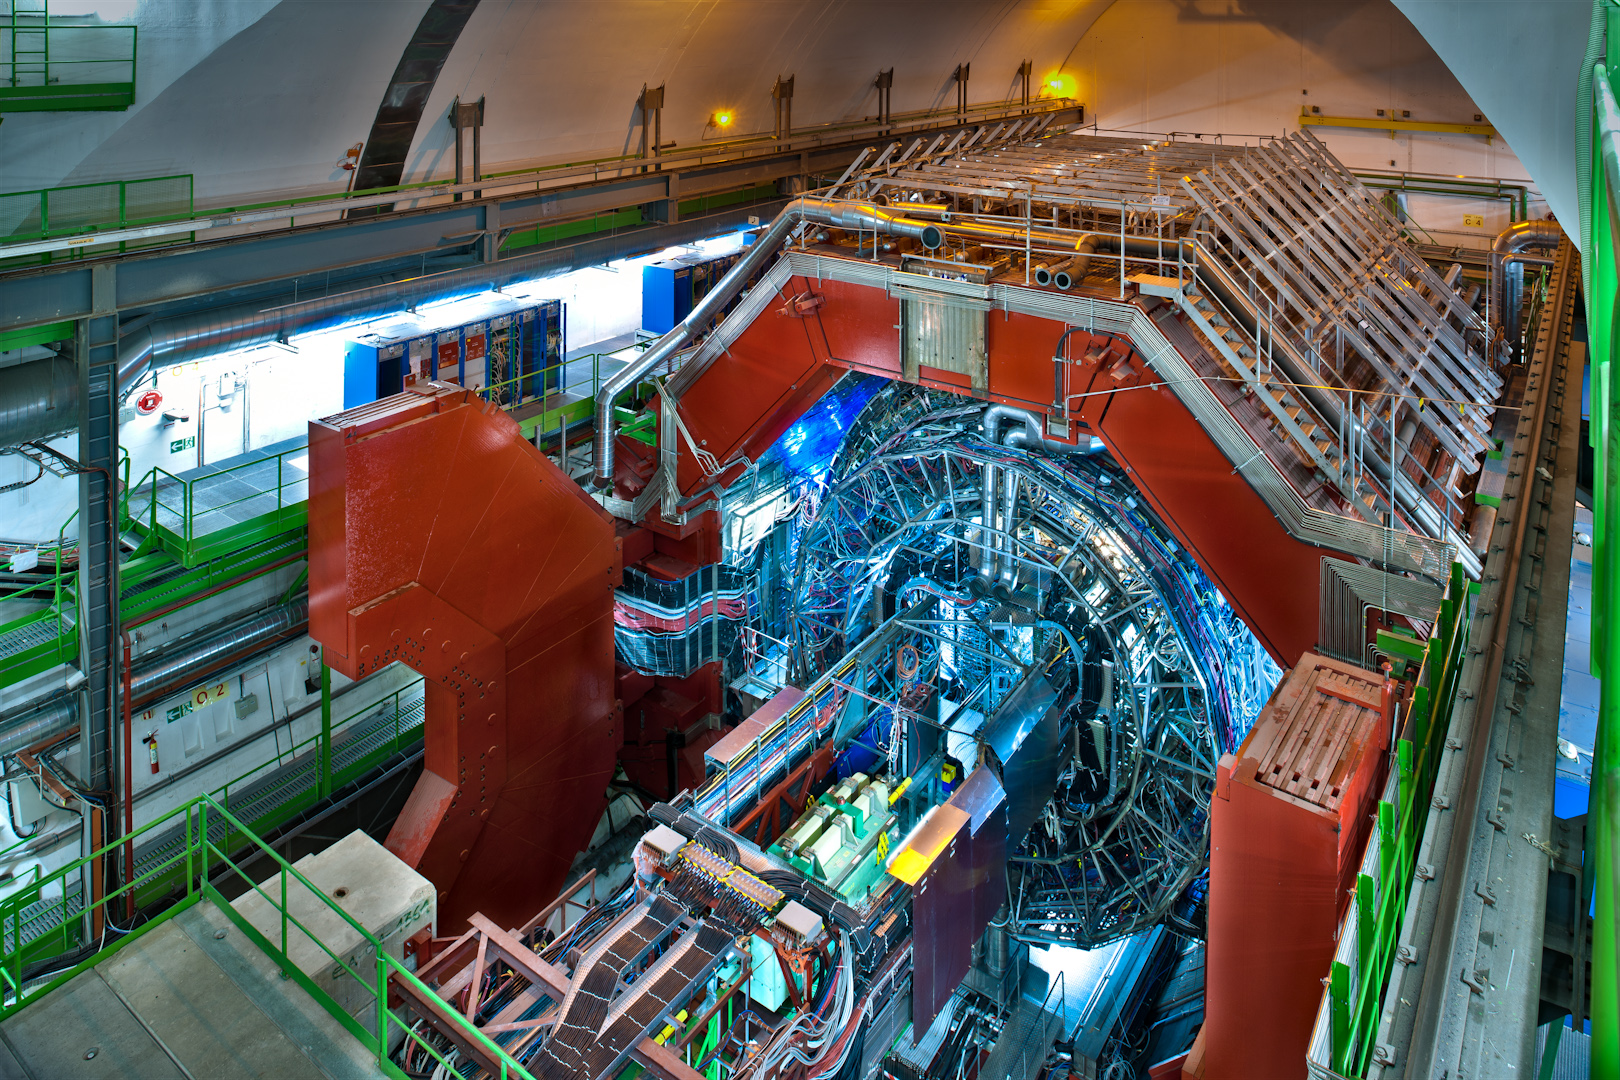
\includegraphics[width=0.6\linewidth]{ALICE/ALICE_LRsaba_CERN_0212_3219.jpg}
        \caption{Foto del rivelatore ALICE}
        \label{fig:ALICEcomplex}
    \end{figure}
    
ALICE \cite{Collaboration_2008_ALICE} è a sua volta composto da vari rivelatori di particelle che permettono di tracciare le traiettorie delle particelle prodotte nella collisione dei fasci, identificarle e misurarne velocità o impulso. I rivelatori di ALICE utilizzati per l'analisi presentata in questa tesi sono descritti nei prossimi paragrafi.

    \subsection{Inner Tracking System (ITS)} \label{ITS}
    L'\textit{Inner Tracking System} è un rivelatore composto da sei cilindri concentrici di rivelatori in silicio di raggio minimo 3.9~cm e massimo 43.0~cm, posizionati con l'asse parallelo alla direzione del fascio. Viene utilizzato per:
    \begin{itemize}
        \item la determinazione della posizione del vertice primario, cioè il punto in cui avviene la collisione dei fasci di protoni; 
        \item la ricostruzione dei vertici secondari di decadimenti di particelle che decadono per interazione debole; 
        \item migliorare la precisione di tracciamento della Time Projection Chamber (TPC) (di cui si parla in seguito nel paragrafo \ref{TPC});
        \item permettere il tracciamento di particelle a basso momento che non vengono tracciate dal rivelatore TPC;
        \item l'identificazione di particelle (PID) con basso impulso trasverso sfruttando la perdita specifica di energia $dE/dx$.
    \end{itemize}
    
    I rivelatori dell'ITS hanno una risoluzione spaziale di poche decine di micrometri. 
    
    \subsection{Time Projection Chamber  (TPC)} \label{TPC}
    La \textit{Time Projection Chamber}  è il principale rivelatore di ALICE per la ricostruzione delle tracce delle particelle prodotte nella collisione. Si tratta di un rivelatore a gas di forma cilindrica, posizionato attorno all'ITS, con raggio interno di 85~cm e esterno di 250~cm e una lunghezza di 500~cm nella direzione del fascio di particelle. Il raggio interno è determinato dalla massima densità di tracce accettabile dalla TPC, quello esterno dalla lunghezza minima necessaria per una precisione del 10$\%$ sulla perdita specifica di energia per ionizzazione $dE/dx$. 
     
     \begin{figure}[htbp]
        \centering
        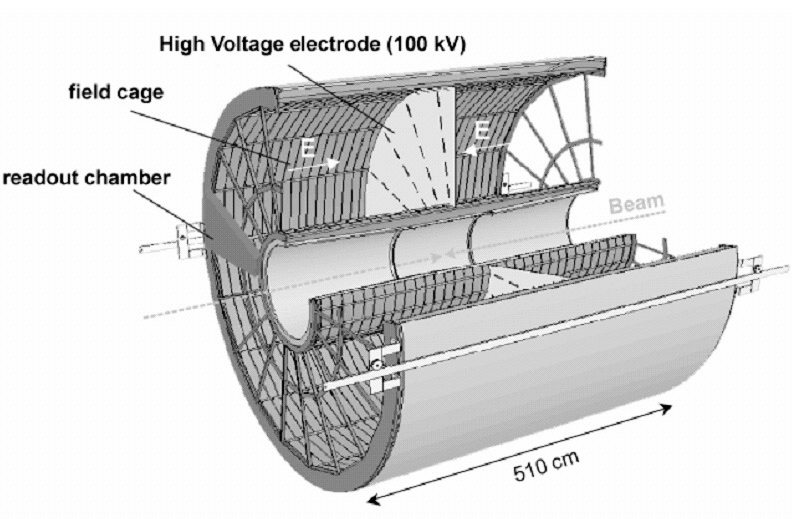
\includegraphics[width=0.7\linewidth]{ALICE/ALICE-TPC-detector.png}
        \caption{Schema della Time Projection Chamber (TPC) di ALICE}
        \label{fig:TPCcomplex}
    \end{figure}
    
    La camera del TPC è riempita con una miscela di gas, che viene ionizzato dal passaggio delle particelle cariche da tracciare. Gli elettroni di ionizzazione vengono accelerati dal campo elettrico creato dagli elettrodi della TPC per arrivare alle placche esterne che permettono di registrare il segnale.
    \\La TPC permette l'identificazione delle particelle tramite la misura della perdita specifica di energia per ionizzazione ($\frac{dE}{dx}$). 
    

    \subsection{Time-Of-Flight (TOF)} \label{TOF}
    Il rivelatore Time-Of-Flight ha forma cilindrica, con raggio minimo di 370 cm e massimo di 399 cm. Questo rivelatore permette l'identificazione delle particelle tramite la misura del tempo di volo dal punto in cui sono state prodotte alla superficie del rivelatore secondo la relazione:
        \begin{equation}
            m = p\sqrt{\frac{t^2_{TOF}}{L^2}-1}
        \end{equation}
    dove $m$ è la massa della particella, $p$ il suo impulso, $t_{TOF}$ il tempo di volo e $L$ la lunghezza della traccia considerata.
    
\chapter{Lo studio dei mesoni conteneti quark charm }

\section{Il Modello Standard}
Per quanto riguarda la fisica delle particelle, il modello che attualmente ne descrive i fondamenti è il \textit{Modello Standard}. In questo modello le particelle fondamentali sono divise tra fermioni e bosoni. 

La figura \ref{fig:ModelloStandard} rappresenta uno schema delle particelle previste dal Modello Standard.
    \begin{figure}[htbp]
        \centering
        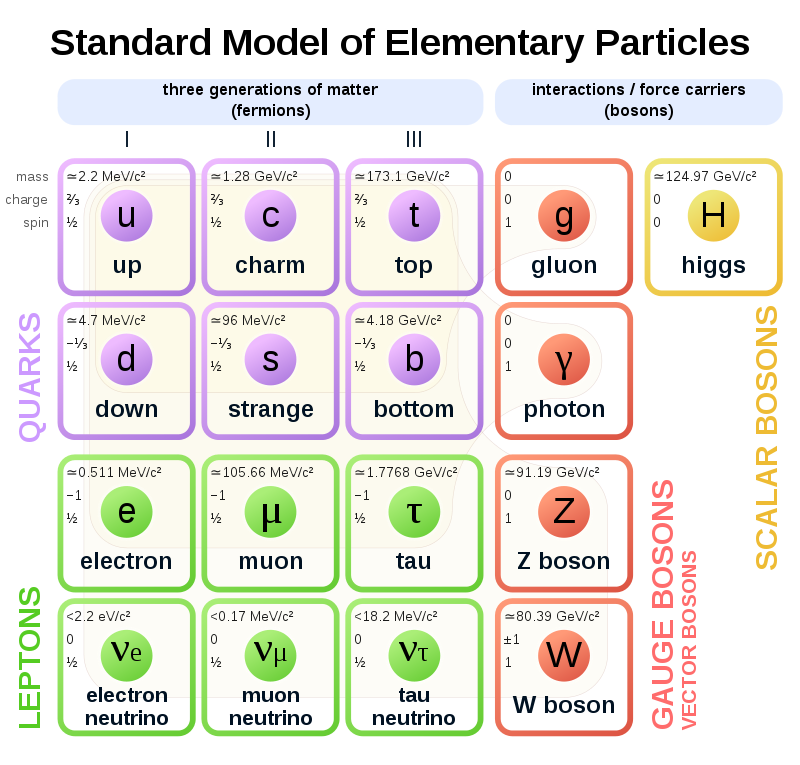
\includegraphics[width=0.65\linewidth]{introParticelle/ModelloStandard.png}
        \caption{Rappresentazione del Modello Standard}
        \label{fig:ModelloStandard}
    \end{figure}
Nella parte sinistra della figura si trovano i \textit{fermioni} divisi tra quark e leptoni. I fermioni sono divisi in tre generazioni ordinate in base a valori di massa crescente. I quark sono contraddistinti dal sapore (up, down, charm, strange, top e bottom) e si combinano per formare barioni (3 quark) o mesoni (coppie di un quark e un anti-quark). Nella parte destra della figura \ref{fig:ModelloStandard} si trovano i \textit{bosoni} che comprendono i bosoni di Gauge, che sono i mediatori delle forze fondamentali previste dal Modello Standard, e il bosone di Higgs, che è l'unico bosone scalare (con spin 0) identificato per la prima volta nel 2012 al Cern. In questa tesi ci si occuper\`a in particolare dei mesoni contenenti un quark charm, la cui importanza e' descritta nel seguito.
 
\section{I mesoni con charm nello studio del QGP}
Il \textit{Plasma di Quark e Gluoni} (QGP) è uno stato della materia in cui i quark e i gluoni non sono confinati negli adroni dalla forza nucleare forte. Gli adroni formati da quark pesanti (come il charm) sono un buono strumento per studiare il QGP formatosi dalla collisione di ioni pesanti. Infatti, il quark charm ha un tempo di formazione pari a $\frac{\hbar}{2m_qc^2} \leq 0.1 \ \mathrm{fm/c} \simeq 0.3 10^{-24}$ s che \`e minore del tempo di formazione del QGP $\simeq (0.3 - 1.5) \ \mathrm{fm/c} \simeq 10^{-24} - 0.5 \ 10^{-23}$ s. Quindi i quark charm, prodotti prima della formazione del QGP, attraversano il QGP stesso e interagiscono con i suoi componenti permettendo di avere informazioni sulle propriet\`a del QGP stesso. Inoltre, i quark pesanti preservano la loro identit\`a mentre attraversano il QGP e infine adronizzano formando adroni che possono essere osservati dai rivelatori di ALICE. I mesoni D, che verranno presi in considerazione in questa tesi, sono formati da un quark charm e un quark pi\`u leggero e costituiscono pertanto delle buone osservabili per lo studio del QGP. 

È di fondamentale importanza studiare la produzione di adroni composti da quark pesanti non solo in collsioni di ioni pesanti, ma anche in collisioni protone-protone in cui non ci si aspetta la formazione del QGP.
Infatti soltanto dal paragone della produzione nei due sistemi \`e possibile ricavare informazioni sull'interazione dei quark charm con il QGP. 
\\Inoltre, la misura di produzione di mesoni D in collisioni protone-protone rappresenta un'ottima verifica per la Cromo-Dinamica Quantistica (QCD), teoria che permette di calcolare la produzione di quark charm e la successiva adronizzazione.

\section{Il mesone $D^{*+}$} \label{mesoneD}
In questa tesi si \`e considerato in particolare il mesone $D^{*+}$, che \`e formato da un quark charm $c$ e un anti-quark down $\overline{d}$ ed ha momento angolare totale 1, e la sua antiparticella $D^{*-}$. Il mesone $D^{*+}$ ha una massa di ($2010.26 \pm 0.05$) MeV/$c^2$ e vita media $ \tau = (7.89 \pm 0.11) {10^{-21}}$~ s~\cite{PDG}. Il decadimento studiato in questa tesi \`e il decadimento forte:
    \begin{equation}
         D^{*+} \rightarrow D^0 + \pi^+ 
    \end{equation}
    che ha un branching ratio BR = $67.7 \%$. 
    Il mesone $D^0$ ha massa $ (1864.83 \pm 0.05)$~ MeV/$c^2$, decade con decadimento debole $D^0 \rightarrow K^- \pi^+$ con un BR = $3.89 \%$ ed ha una vita media di $(410.1 \pm 1.5 ) 10^{-15}$~s~\cite{PDG}.
\\Nel caso in cui la $D^{*+}$ decada da ferma, il pione ha un impulso di soli $39$ MeV/c e veine indicato come $\pi_{soft}$. \\Il Q-valore del decadimento \`e:
    \begin{equation}
        Q = m_{D^{*+}} - (m_{D^{0}} + m_{\pi_{soft}}) = 5.93 \ \mathrm{MeV/c^2}
    \end{equation}

La figura \ref{fig:decadimentoD} rappresenta la topologia del decadimento del mesone $D^{*+}$. Il punto di decadimento della $D^{*+}$ \`e indistinguibile dal vertice primario, ovvero il punto in cui avviene la collisione dei fasci di protoni, a causa delle distanze che caratterizzano il decadimento forte. Il pione $\pi_{soft}$ emesso dal decadimento del mesone $D^{*+}$ viene direttamente rivelato dai rivelatori di ALICE. Il punto di decadimento del mesone $D^0$ (che decade con decadimento debole) \`e, invece, separato dal vertice primario di $c\tau = 122.9 \ \mu m $, dove $c$ \`e la velocit\`a della luce nel vuoto e $\tau$ la vita media del mesone $D^0$. Il punto di decadimento del mesone $D^0$ viene chiamato vertice secondario (SV).
 
    \begin{figure}[htbp]
        \centering
        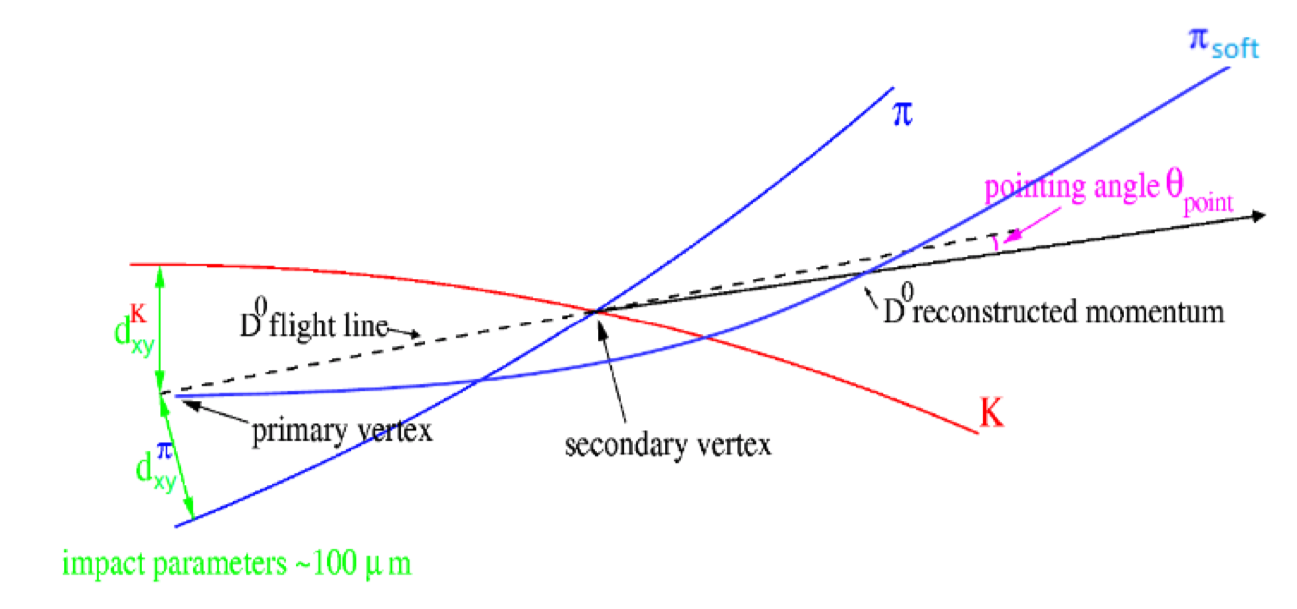
\includegraphics[width=0.9\linewidth]{introParticelle/DecadimentoDStar.png}
        \caption{Topologia del decadimento del mesone $D^{*+}$ nel canale $D^{*+} \rightarrow D^0 \pi^+$ e successivo decadimento $D^0 \rightarrow K^- \pi^+$. Il vertice di decadimento del mesone $D^{*+}$ \`e indistinguibile dal vertice primario a causa delle distanze caratteristiche dei decadimenti forti}
        \label{fig:decadimentoD}
    \end{figure}
    
Per identificare il mesone $D^{*+}$, inizialmente, si ricostruiscono le candidate $D^0$ considerando tutte le possibili combinazioni di due tracce di segno opposto. Successivamente le candidate $D^0$ cos\`i ricostruite vengono combinate con la traccia di un candidato pione. Per ridurre il fondo combinatoriale costituito dalle coppie $\pi^+ \ K^-$ che non vengono dal decadimento di un mesone $D^0$, vengono applicate delle selezioni sulle variabili topologiche.
\\Tali variabili topologiche sono riportate in figura \ref{fig:decadimentoD} e sono:
    \begin{itemize}
        \item la lunghezza di decadimento della $D^0$, ovvero la distanza tra il vertice primario e secondario;
        \item i parametri d'impatto del kaone e del pione (in figura \ref{fig:decadimentoD} indicati come ${d^K}_{XY}$ e ${d^\pi}_{XY}$ rispettivamente per kaone e pione), che sono la distanza minima tra la traiettoria di kaone o pione e il vertice primario;
        \item l'angolo di puntamento, indicato come $\theta_{point}$, che \`e l'angolo tra la retta congiungente il PV e il SV e la direzione del vettore impulso trasverso ($p_T$) della candidata $D^{0}$ ricostruita;
        \item l'angolo di decadimento, che \`e l'angolo tra il vettore impulso del mesone $D^0$ e il vettore impulso del $\pi^+$ nel sistema di riferimento della candidata $D^0$ ricostruita;
        \item la distanza di minimo approccio (DCA), ovvero la distanza minima tra le traiettorie del $K^-$ e del $\pi^+$ nel piano perpendicolare alla direzione del fascio.
    \end{itemize}{}

In aggiunta alla selezione sulle variabili topologiche, viene anche utilizzata l'identificazione di particelle con TPC e TOF per identificare il pione e il kaone derivanti dal decadimento del mesone $D^0$.
\\Nell'analisi standard di ALICE le selezioni sulle variabili topologiche indicate sopra vengono ottimizzate con una procedura manuale per massimizzare la quantit\`a di segnale rispetto al fondo combinatoriale. Nel lavoro presentato in questa tesi, l'analisi multivariata implementata nell'algoritmo del Boosted Decision Tree combina le variabili topologiche creando un'unica variabile discriminatoria finale.
\\Per determinare il numero di candidate $D^{*+}$ ricostruite  si utilizza un'analisi in massa invariante, quest'ultima \`e definita come: 
    \begin{equation}
        M = {E^2}_{TOT} - {p^2}_{TOT}
    \end{equation}
dove $E_{TOT}$ \`e l'energia totale di tutte le particelle del sistema considerato e $p_{TOT}$ \`e l'impulso totale. 
\\Nel caso della $D^0$ la massa invariante del doppietto pione-kaone \`e data da:  
    \begin{equation}
        M(K^- \pi^+) = ({E_{\pi^+}+E_{K^-}})^2 - ({p_{\pi^+}+p_{K^-}})^2
    \end{equation}
dove $E_{\pi^+}$ e $E_{K^-}$ sono le energie del pione e del kaone, $p_{\pi^+}$ e $p_{K^-}$ sono i rispettivi impulsi.
\\La massa invariante della candidata $D^{*+}$ \`e data da:
    \begin{equation}
        M(K^- \pi^+ \pi_{soft}) = ({E_{\pi^+}+E_{K^-}+E_{\pi_{soft}}})^2 - ({p_{\pi^+}+p_{K^-}+p_{\pi_{soft}}})^2
    \end{equation}
Dove $E_{\pi_{soft}}$ \`e l'energia del $\pi_{soft}$ e $p_{\pi_{soft}}$ il suo impulso.
\\Il segnale relativo al mesone $D^{*+}$ si studia preferibilmente usando la variabile $\Delta M$
  \begin{equation}
       \Delta M = M (K^- \pi^+ \pi^+) - M(K^- \pi^+)
    \end{equation}
    
dove $ M (K^- \pi^+ \pi^+)$ \`e la massa invariante ricostruita della candidata $D^{*+}$ e $ M(K^- \pi^+)$ la massa invariante ricostruita della candidata $D^{0}$. La distribuzione della variabile $\Delta M$ mostra un picco al valore di circa $145$~ MeV/c. Si considera preferibilmente la distribuzione di $\Delta M$ in quanto nella sottrazione l'incertezza sull'impulso del kaone e del pione si cancellano e la larghezza del picco \`e determinata solo dalla risoluzione sull'impulso del $\pi_{soft}$. La figura \ref{fig:distribuzione_massa} mostra un esempio della distribuzione della differenza di massa invariante $\Delta M$ per candidate $D^{*+}$ con un impulso trasverso $p_T$ [3,4] GeV/c selezionate con l'analisi multivariata, come verr\`a spiegato nel capitolo \ref{applicazione}. A destra del picco di segnale \`e visibile il fondo combinatoriale. Su questo grafico si far\`a poi un fit sia del picco di segnale, sia del fondo per ottenere la quantit\`a di $D^{*+}$ selezionata. 

    \begin{figure}[htbp]
        \centering
        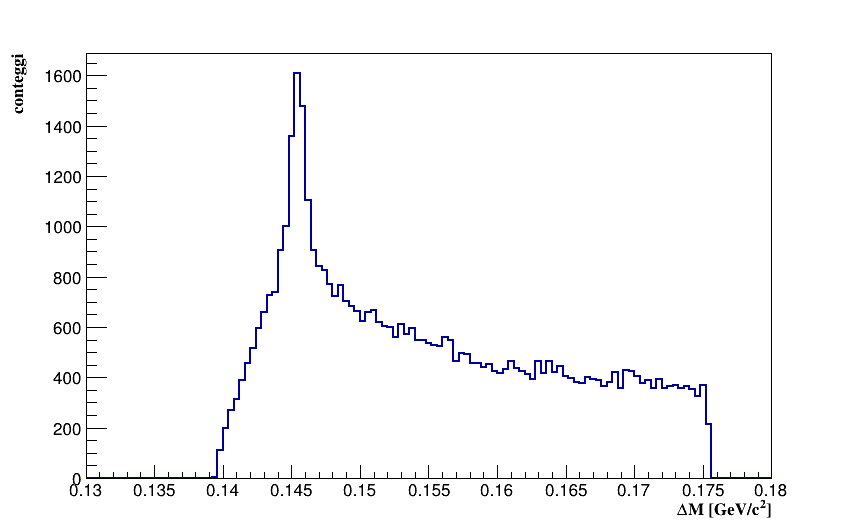
\includegraphics[width=0.8\linewidth]{AnalisiDati/diffDstarD0_3_4BDT.png}
        \caption{Distribuzione di massa invariante $\Delta M = M (K^- \pi^+ \pi^+) - M(K^- \pi^+)$ del campione di dati di ALICE nell'intervallo di impulso trasverso $p_T$ [3,4] GeV/c dopo l'applicazione dell'algoritmo BDT.}
        \label{fig:distribuzione_massa}
    \end{figure}




\chapter{Introduzione ai Boosted Decision Tree}

In questa tesi l'analisi dati per la selezione del mesone $D^{*+}$ \`e stata svolta utilizzando algoritmi di machine learning (apprendimento artificaile).\footnote{machine larning: meccanismo che permette ad una macchina intelligente di migliorare le proprie prestazioni nel tempo. \cite{sitoMachineLearning}} Questo per confrontare i risultati ottenuto con questo metodo con quelli dell'analisi standard di ALICE. In questo capitolo si illustrano pertanto le caratteristiche principali dell'algoritmo di machine learning utilizzato.  

\section{Analisi Multivariata e Problemi di Selezione} \label{AnalisiMulti}
Il machine learning consiste nello sviluppo di algoritmi che possono imparare dai dati e in base ad essi prendere decisioni o fare previsioni. Il machine learning può essere di tipo supervisionato o non supervisionato. Nel primo caso si utilizzano degli esempi per addestrare l'algoritmo di cui si fornisce anche la "risposta". In questo modo vi è una sorta di feedback su cui si basa l'addestramento. Nel caso non supervisionato, al contrario, vengono forniti solo dei dati e sarà l'algoritmo stesso a decidere indipendentemente come classificarli. L' \textit{analisi multivariata}  appartiene al caso del machine learning supervisionato. Prevede, infatti, che tutte le variabili vengano combinate (in base al metodo scelto) in un'unica variabile finale, chiamata \textit{classifier output}, che fornisce il metodo di valutazione finale.
\\In questa tesi si affronta un \textit{problema di selezione}, ovvero si cerca un segnale raro in un insieme composto principalmente da eventi di fondo, per cui il rapporto segnale su fondo \`e basso.
Per l'analisi svolta in questa tesi \`e stato utilizzato il "TMVA" (Tool for MultiVariate Analysis), che \`e uno strumento incluso in Root che implementa diversi metodi di analisi multivariata. L'analisi effettuata si struttura in due fasi principali:
    \begin{itemize}
        \item Training: in questa fase l'algoritmo analizza dati di cui conosce gi\`a il tipo e li utilizza per apprendere quali sono le caratteristiche dei vari tipi di dati;
        \item Applicazione: nella fase di applicazione viene utilizzato quanto appreso dalla macchina nella fase di training per selezionare e dividere dati di cui non si conosce il tipo.
    \end{itemize}
    
\section{Boosted Decision Tree} \label{BDT}

    \subsection{Alberi decisionali}
    Un \textit{albero decisionale} (decision tree) è una struttura che classifica i dati mediante scelte di tipo binario. Se ne riporta un esempio base in figura \ref{fig:BDT}. Ogni scelta è basata su una selezione su una singola variabile. %Ogni scelta è basata su un taglio su una singola variabile.
    Ogni ramo creato viene poi nuovamente diviso in due in base al taglio su un'altra variabile. I gruppi di dati creati alla fine dell'albero sono chiamati foglie. Queste vengono selezionate come segnale o background in base alla classe cui appartiene la maggior parte degli eventi. 
    
    \begin{figure}[htbp]
        \centering
        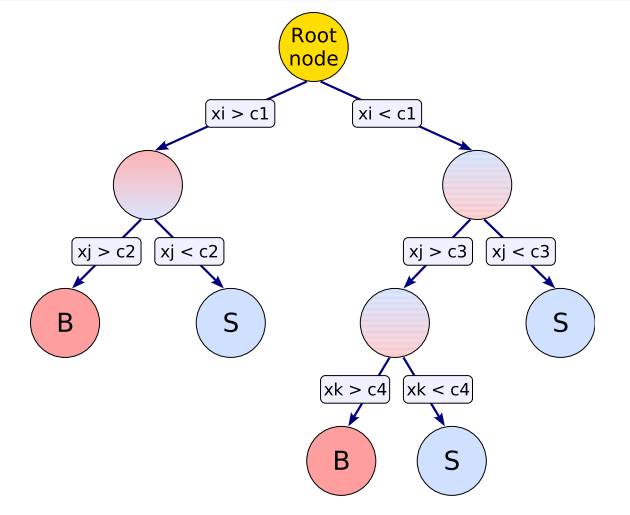
\includegraphics[width=0.5\linewidth]{TMVA/BDT1.PNG}
        \caption{ Esempio di schema di un decision tree}
        \label{fig:BDT}
    \end{figure}
    
    Un vantaggio dei decision tree è che sono facilmente visualizzabili ed è altrettanto semplice ricondursi al significato fisico dei tagli operati. Inoltre sono perlopiù insensibili alla presenza di variabili poco discriminanti (cosa che non accade, invece, per molte altre tecniche di analisi multivariata). Lo svantaggio principale è che sono fortemente sensibili alle fluttuazioni statistiche dei dati utilizzati per il training. Questo problema viene risolto con il "boosting" di cui si parla nella sezione  \ref{Boosting}.
    \\Per poter creare il decision tree \`e necessario un set di dati per il \textit{training}, ovvero dei dati di cui si consce già se siano segnale o fondo. La prima divisione dei dati, chiamata root node, viene scelta individuando la variabile e il suo relativo taglio che meglio divide i dati tra segnale e background. L'indice di separazione utilizzato in questa tesi è quello di Gini \footnote{L'indice di Gini è definito come: $p (1-p)$, dove $p$ è la purezza del segnale, che è il rapporto tra il numero di eventi segnale e il numero di eventi totale}. A questo punto si considera singolarmente ognuno dei due rami e si sceglie il taglio sulla variabile che massimizza l'aumento dell'indice di separazione. Si continua così finchè non viene raggiunto uno dei criteri di stop,  a questo punto la struttura dell'albero è formata ed è possibile verificare in che modo sono stati divisi i dati tra segnale e background. 
    \\Infine è necessario fare un controllo per l'\textit{overtraining}, ovvero la possibilità che il decision tree si sia sensibilizzato eccessivamente al set di dati utilizzati nella fase di training e non sia più descrittivo del fenomeno fisico nella sua generalità. Per fare ciò si utilizzano dei dati generati da simulazione, che però non sono stati utilizzati nella fase di training e si controlla che la risposta del decision tree sui dati del training e su questi nuovi dati (detti dati del testing) sia simile.\cite{TMVAGuide} 
 
    \subsection{Boosting} \label{Boosting}
    Per migliorare le performance dell'algoritmo di amchine learning \`e utile utilizzare il meccanismo del \textit{boosting}. Questo viene utilizzato nel caso dei decision tree per renderli più stabili rispetto alle fluttuazioni statistiche del set di dati del training e per migliorarne la capacit\`a di selezionare i dati. Per fare ciò l'algoritmo ripete automaticamente il training pi\`u volte utilizzando lo stesso set di dati e ad ogni ripetizione d\`a pesi diversi ai dati.
    \\L'algoritmo di boosting utilizzato in questa tesi è l'\textit{Adaptive Boosting} (AdaBoost). In questo caso i dati che sono stati classificati erroneamente nel precedente decision tree vengono ripesati con un fattore $\alpha$, che è calcolato come 
        \begin{equation}
            \alpha = \frac{1 - err}{err}
        \end{equation}
    Dove $err$ è il rate di eventi classificati erroneamente. 
    \\Si viene a creare una foresta di decision tree da cui si deriva il responso finale per la selezione degli eventi. Gli algoritmi di boosting funzionano meglio se si utilizzano alberi piccoli, ovvero con pochi livelli di diramazione.
    Utilizzando questa tecnica, pertanto, si riesce a rendere l'algoritmo più stabile ed efficiente ma d'altra parte si perde il senso fisico della selezione tra segnale e fondo. 
    
    
    
    

\chapter{Training e Testing del BDT}

\section{I Dati inziali}

I dati utilizzati per l'analisi svolta sono relativi a collisioni di due fasci di protoni incidenti al Cern. I dati racccolti neò 2017 da ALICE sono caratterizzati da un valore di $\sqrt{s} = 5 \ TeV$ \footnote{s è la massa inavriante della collisione, definita come $s = E^2 - \bar p ^2$} e sono relativi a 985 milioni di collisioni.
\\Da questi dati si vogliono selezionare solo le $D^{*+}$, che sono state ricostruite dal decadimento $D^{*+} \rightarrow D^0 + \pi^+ $ di cui si è parlato nel \ref{mesoneD}. Per fare ciò ai dati utilizzati sono già state applicate delle pre-selezioni estremamente morbide che permettono di preservare praticamente tutto il segnale e di fare una prima scrematura dei dati grezzi.
A questo punto tutta l'analisi che segue è stata svolta considerando i dati suddivisi in vari intervalli. La suddivisione è basata sul valore del $p_T$, che è il valore del momento trasverso, ovvero il momento nella direzione perpendicolare a quella dei fasci di particelle incidenti. Gli intervalli inizialmente considerati sono: [1,2], [2,3], [3,4], [4,5], [5,6], [6,8], [8,12], [12,16], [16,24] misurati in GeV/c. 
\\Per poter visualizzare i dati si possono considerare gli istogrammi della massa della $D^{*+}$, nel nostro caso si è scelto di utilizzare gli istogrammi della differenza in massa tra la $D^{*+}$ e la $D^0$ prodotta nel decadimento. Questa differenza in massa non è altro che la massa del $\pi^+$ relativo al primo decadimento, anche detto soft pi, che è il pione con momento più basso (rispetto al $\pi^+$ prodotto nel decadimento della $D0$) ed è misurata in $Gev/c^2$. %Come mai usiamo gli istogrammi della differenza in massa e non direttamente quelli della massa della Dstar??
Di seguito si riportano gli istogrammi relativi ad alcuni intervalli di $p_T$, quelli relativi agli altri intervalli di $p_T$ si trovano in appendice. 

    \begin{figure}[htbp]
        \centering
        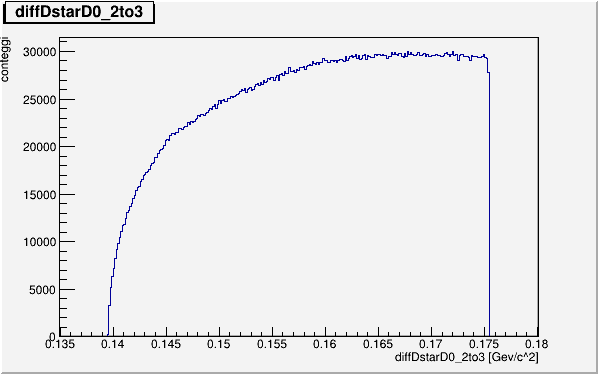
\includegraphics[width=0.7\linewidth]{training&testing/diffDstarD0_2to3.png}
        \caption{}
        \label{fig:grafmassDstar1}
    \end{figure}
    
Come si può vedere dal grafico \ref{fig:grafmassDstar1} non si evidenzia nessun picco evidente, cosa che ci si aspetta nel caso di una risonanza come la $D^{*+}$.\footnote{Una risonzanza è una particella che ha un tempo di vita così corto da non essere direttamente osservabile e la cui esistenza si evidenzia considerando i prodotti del suo decadimento. In questo caso si vede un aumento della probabilità di trovare i prodotti del decadimento della risonanza in corrispondenza del valore della massa invariante della risonanza stessa} Questo accade perchè il numero di $D^{*+}$ prodotte è troppo piccolo rispetto al fondo di altre particelle e pertanto il picco della $D^{*+}$ non è riconoscibile rispetto al background.

    \begin{figure}[htbp]
        \centering
        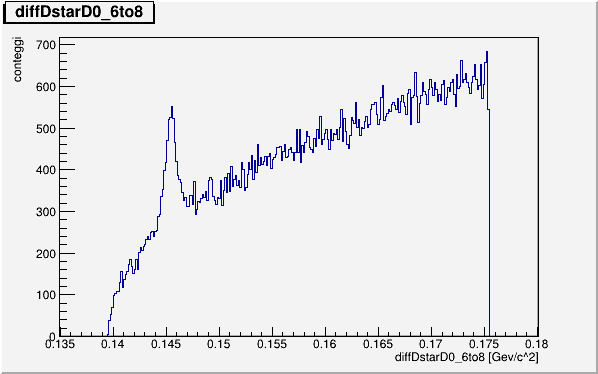
\includegraphics[width=0.7\linewidth]{training&testing/diffDstarD0_6to8.png}
        \caption{}
        \label{fig:grafmassDstar2}
    \end{figure}


Diversamente accade nel caso del grafico \ref{fig:grafmassDstar2} in cui si considera un intervallo di $p_T$ con valori del momento trasverso più alti. In questo caso il picco della $D^{*+}$ è già visibile e riconoscibile rispetto al fondo. 
La differenza dei grafici si riscontra per tutti gli intervalli di $p_T$ e tanto più è alto il $p_T$ tanto più è evidente il picco. Per ricostruire la $D^{*+}$ si considerano le combinazioni di tracce di due $\pi^+$ e un $K^-$ , ma a basso $p_T$ ci sono più combinazioni possibili mentre ad alto $p_T$ ce ne sono di meno. Pertanto per valori del momento trasverso più bassi le combinazioni errate, ovvero non relative alla $D^{*+}$ sono di più e quindi il fondo stesso è maggiore a basso $p_T$.

    \subsection{Le variabili di taglio}
    La selezione di tipo standard che viene svolta ad ALICE per il riconoscimento delle $D^{*+}$ è basata sulla scelta di alcune variabili di taglio e per ognuna di queste si sceglie un valore di \textit{cut}. Le \textit{variabili di taglio} sono grandezze fisiche che descrivono il decadimento della $D^{*+}$ e che permettono di comprendere se le particelle considerate sono i prodotti di quel decadimento o meno. Il cut, invece, è il valore scelto per discriminare tra segnale e background. 
    \\Anche per utilizzare il metodo del BDT sono state scelte alcune variabili di taglio, da cui, poi, l'algoritmo del BDT ha ricavato un'unica variabile finale: il textit{classifier output}. Solo per quest'ultima variabile è stato scelto un valore di cut in base a cui selezionare le candidate $D^{*+}$. 
    Le variabili di taglio che possono essere considerate sono le seguenti:
        \begin{itemize}
            \item \textbf{massa$\bm{D^{*+}}$} è la massa della $D^{*+}$
            \item \textbf{massa$\bm{D^0}$} è la massa della $D^0$
            \item \textbf{diff$\bm{D^{*+}D^0}$} è la differenza tra la massa della  $D^{*+}$ e della $D^0$
            \item \textbf{$\bm{p_TD^{*+}}$} è il momento trasverso della $D^{*+}$
            \item \textbf{$\bm{{p_T\pi^+}_{soft}}$} è il momento trasverso del $\pi^+$ soft
            \item \textbf{$\bm{p_T\pi^+}$} è il momento trasverso del $\pi^+$ soft 
            \item \textbf{$\bm{p_TK^-}$} è il momento trasverso del $K^-$
            \item \textbf{$\bm{\eta}$} è l'angolo tra la direzione dei fasci di protoni incidenti e la direzione in cui è prodotta la $D^*+$ %Controllare se è giusto!!!
            \item \textbf{dist$\bm{K^-}$} è la distanza tra la traiettoria del Kaone $K^-$ e il vertice primario (PV) % \footnote{Il vertice primario è il punto in cui decade la $D^*+$}
            \item \textbf{dist$\bm{\pi^+}$} è la distanza tra la traiettoria del $\pi^+$ (prodotto dal decadimento della $D^0$) e il PV
            \item \textbf{distdist} è il prodotto $d0K \ d0Pi$
            \item \textbf{DCA} ovvero Distance of Closest Approach, è la distanza minima tra le traiettore del $K^-$ e del $\pi^+$, in teoria questa distanza dovrebbe essere nulla, in quanto le due traiettorie si dovrebbero incontrare nel vertice secondario (SV) %\footnote{Il vertice secondario è il punto in cui decade la $D^0$}.
            \item \textbf{cos$\bm{\theta_P}$} è il coseno dell'angolo di pointing. Quest'ultimo è l'angolo tra la retta congiungente il PV e il SV e la direzione del $p_T$ della $D^{*+}$.
             \item \textbf{cos$\bm{\theta_{P_{XY}}}$} è la proiezione del cos$\theta_P$ sul piano perpendicolare alla direzione dei fasci di protoni
            \item \textbf{cos$\bm{\theta^*}$} 
            \item \textbf{cos$\bm{\bar \theta^*}$}
            \item $\bm{\theta}$ 
            \item $\bm{L_{DECAD}}$ è la distanza di volo (ovvero la lunghezza di decadimento) della $D^0$ normalizzata per il suo errore 
             \item $\bm{L_{{DECAD}_{XY}}}$ è la proiezione della $\bm{L_{DECAD}}$ sul piano perpendicolare alla direzione dei fasci di protoni
        \end{itemize}{}
       
        
   Queste sono le variabili di taglio scelte inizialmente per il training del BDT. Dalle \textit{simulazioni Monte Carlo} si può vedere che queste variabili hanno una distribuzione diversa nel caso si consideri il segnale o il fondo. Proprio in base a queste differenze l'algoritmo utilizzato per questa analisi costruisce il BDT fornendo, alla fine del training, il classifier output. Si riportano di seguito i grafici delle distribuzioni di alcune di queste variabili per i dati (ottenuti da ALICE), per la simulazione del segnale e per la simulazione del fondo (ottenuti da simulatore MonteCarlo).
   
    \begin{figure}[htbp] %inserire grafici cca 4 variabili di taglio
        \centering
        \includegraphics[width=0.7\linewidth]{training&testing/variabilitaglio.png}
        \caption{}
        \label{fig:variabilitaglio}
    \end{figure}
   
   
    Durante la fase iniziale, si è provato il training del BDT utilizzando diversi set di variabili di taglio. In particolare si è considerata la correlazione tra le variabili, che può peggiorare i risultati degli algoritmi di analisi multivariata. Si è quindi scelto di non considerare le variabili fortemente correlate tra loro, dato che, nel caso in analisi, eliminare queste variabili non va a diminuire l'efficienza dell'algoritmo di training. 
    
    \begin{minipage}{.5\textwidth}%{0.5 cm} 
        \begin{flushleft} \large
        \flushleft
        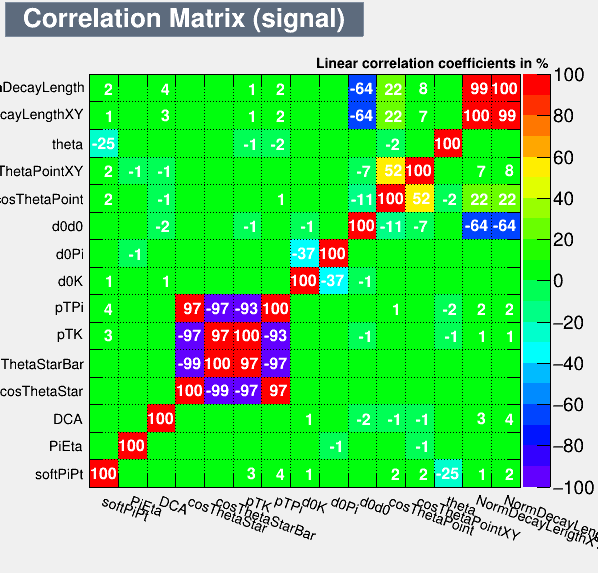
\includegraphics[width=7.5cm]{training&testing/CorrelationMatrixSin.png}
        \captionof{figure}{Griglia che mostra la correlazione lineare in percentuale tra le variabili di taglio considerate inizialmente per il training per il segnale (da simulazione Monte Carlo)}
        \label{fig:correlazInizialeS}
        \end{flushleft}
        \end{minipage}
    ~
    \begin{minipage}{0.5\textwidth}
        \begin{flushright} 
        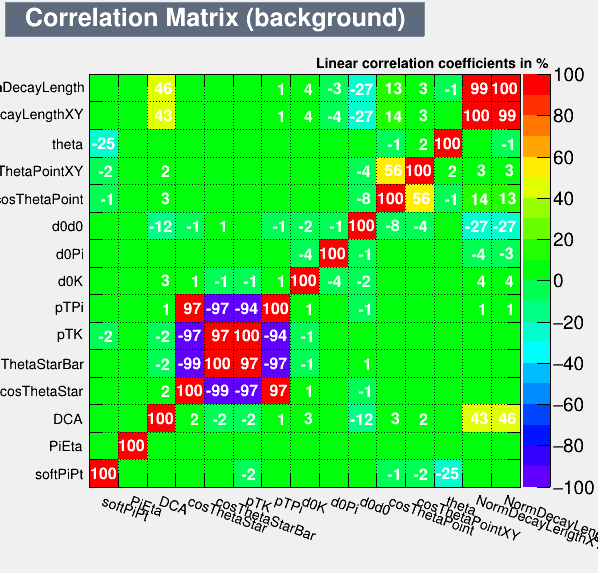
\includegraphics[width=7.5cm]{training&testing/CorrelationMatrixBin.png}
        \captionof{figure}{Griglia che mostra la correlazione lineare in percentuale tra le variabili di taglio considerate inizialmente per il training per il fondo (da simulazione Monte Carlo)}
        \label{fig:correlazInizialeB}
        \end{flushright}
    \end{minipage}\\[0.5cm]
    
 %   \begin{figure}[htbp] %grafico correlazione lineare tutte variabili
 %       \centering
 %       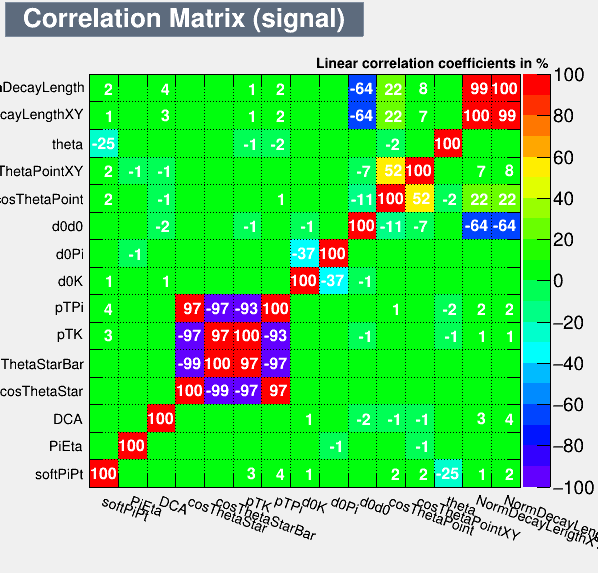
\includegraphics[width=0.7\linewidth]{training&testing/CorrelationMatrixSin.png}
%        \caption{Griglia che mostra la correlazione lineare in percentuale tra le variabili di taglio considerate inizialmente per il training per il segnale (da simulazione Monte Carlo)}
%        \label{fig:correlazInizialeS}
%    \end{figure}
    
    
%     \begin{figure}[htbp] %grafico correlazione lineare tutte variabili
%        \centering
%        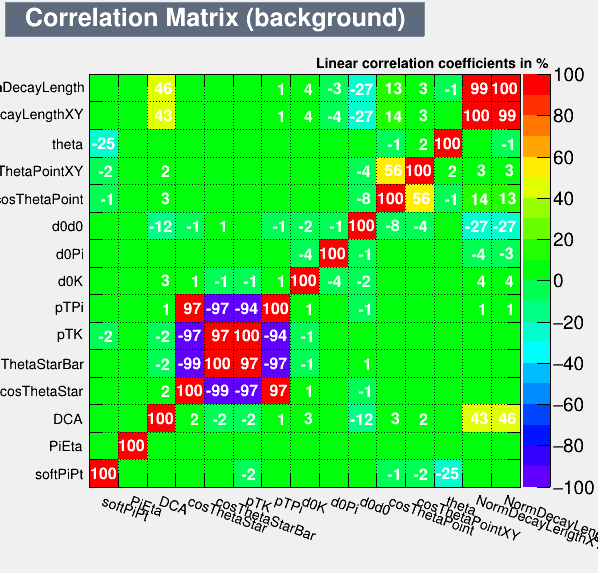
\includegraphics[width=0.7\linewidth]{training&testing/CorrelationMatrixBin.png}
%        \caption{Griglia che mostra la correlazione lineare in percentuale tra le variabili di taglio considerate inizialmente per il training per il fondo (da simulazione Monte Carlo)}
%        \label{fig:correlazInizialeB}
%    \end{figure}
    
    
    Inoltre si è deciso di aggiungere anche la \textit{Particle Identification} (PID), che ha permesso di ottenere risultati migliori nella fase di analisi dei dati di ALICE. La PID sfrutta i dati relativi alla perdita di energia delle particelle all'interno del rivelatore: $\frac{dE}{dx}$. Conoscendo la carica della particella e le caratteristiche del materiale di cui è composto il rivelatore, si può utilizzare la \textit{Bethe-Bloch}. Confrontando i dati della perdita di energia con la Bethe-Bloch si può ricavare la massa della particella e quindi identificare la particella stessa. In pratica le limitazioni dovute alle fluttuazioni statistiche e alla precisione dei rivelatori non permettono un'identificazione certa ma di tipo statistico. 
    \\Allo stesso modo è stato utilizzato anche il \textit{Time Of Flight} (TOF), ovvero la misura del tempo impiegato dalla particella a percorrere una determinata lunghezza nel rivelatore. Conoscendo la lunghezza considerata e il momento della particella si può ricavare la massa della particella stessa. Anche in questo caso le stesse limitazioni della PID impediscono un'identificazione diretta e certa della particella. 
    
    \begin{figure}[htbp]
        \centering
        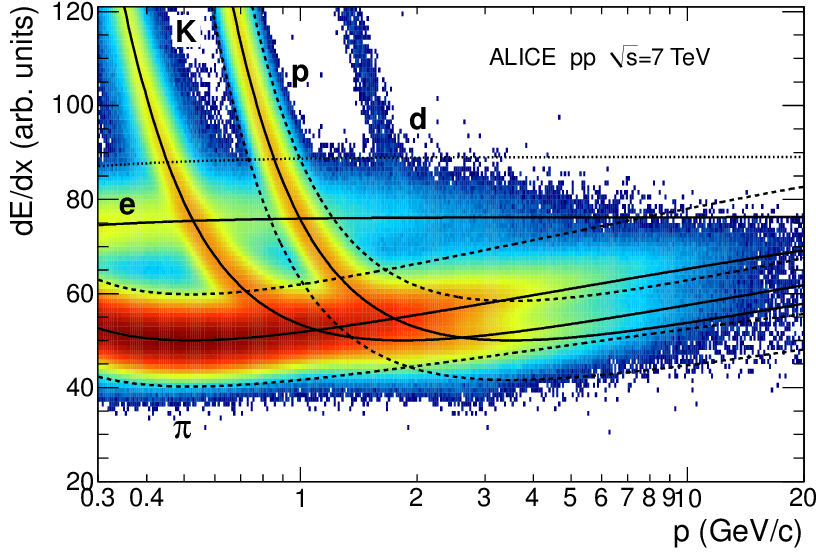
\includegraphics[width=0.6\linewidth]{training&testing/Specific-energy-loss-in-the-TPC.png}
        \caption{ Perdita di energia specifica nella TPC (\ref{TPC}) in funzione del momento, sono riportati anche gli andamenti della Bethe-Bloch per vari tipi di particelle.}
        \label{fig:BBnellaTPC}
    \end{figure}
    
    Come si vede dalla figura \ref{fig:BBnellaTPC}, i dati non possono sempre essere ricondotti univocamente all'andamento di una singola particella. Nell'analisi relativa a questa tesi si è considerata la differenza tra la $\frac{dE}{dx}\mid_m$ misurata dalla TPC e la $\frac{dE}{dx}\mid_{th}$ calcolata con la Bethe-Bloch, il tutto rinormalizzato per la risoluzione della TPC. 
    \\Allo stesso modo è stata utilizzata anche la differenza tra il $TOF\mid_{m}$ misurato con il rivelatore TOF e il $TOF\mid_{th}$ calcolato terociamente, tutto rinormalizzato per la risoluzione del rivelatore TOF.
    
    Le variabili di taglio aggiunte sono:
    \begin{itemize}
        \item $\bm{TPC_{PID,\pi^+}}$: $(\frac{dE}{dx}\mid_{m, \pi} \ - \ \frac{dE}{dx}\mid_{th, \pi} ) / \sigma_{TPC} \ $ per il $\pi^+$ prodotto dal decadimento della $D^0$ %nSigmaTPCpi
        \item $\bm{TPC_{PID,K^-}}$ :  $(\frac{dE}{dx}\mid_{m,K} \ - \ \frac{dE}{dx}\mid_{th,K} ) / \sigma_{TPC} \ $ per il $K^-$ prodotto dal decadimento della $D^0$ %nSigmaTPCK
        \item $\bm{TOF_{PID,\pi^+}}$ : $ (TOF\mid_{m,\pi} \ - \ TOF\mid_{th,\pi}) / \sigma_{TOF} \ $ per il $\pi^+$ prodotto dal decadimento della $D^0$ %nSigmaTOFpi
        \item $\bm{TOF_{PID,K^-}}$ : $ (TOF\mid_{m,K} \ - \ TOF\mid_{th,K}) / \sigma_{TOF} \ $ per il $K^-$ prodotto dal decadimento della $D^0$ %nSigmaTOFK
    \end{itemize}{}
    
    La correlazione tra le variabili utilizzate per l'analisi dei dati finale di ALICE è minima per tutte le variabili, ad eccezione delle variabili $L_{{DECAD}_{XY}}$ , distdist, e DCA, come si vede dalle figure \ref{fig:correlazFinaleS} e \ref{fig:correlazFinaleB}
   
      \begin{minipage}{.5\textwidth}%{0.5 cm} 
        \begin{flushleft} \large
        \flushleft
        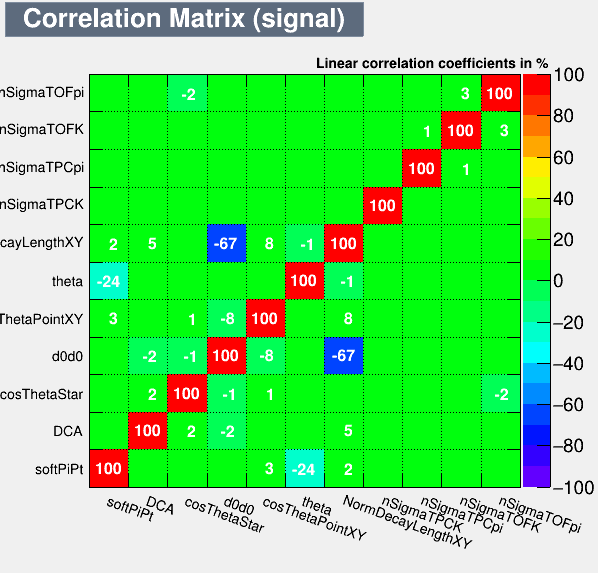
\includegraphics[width=7.5cm]{training&testing/CorrelationMatrixS.png}
        \captionof{figure}{Correlazione lineare in percentuale tra le variabili di taglio considerate per il training finale del segnale (da simulazione Monte Carlo)}
        \label{fig:correlazFinaleS}
        \end{flushleft}
        \end{minipage}
    ~
    \begin{minipage}{0.5\textwidth}
        \begin{flushright} \large
        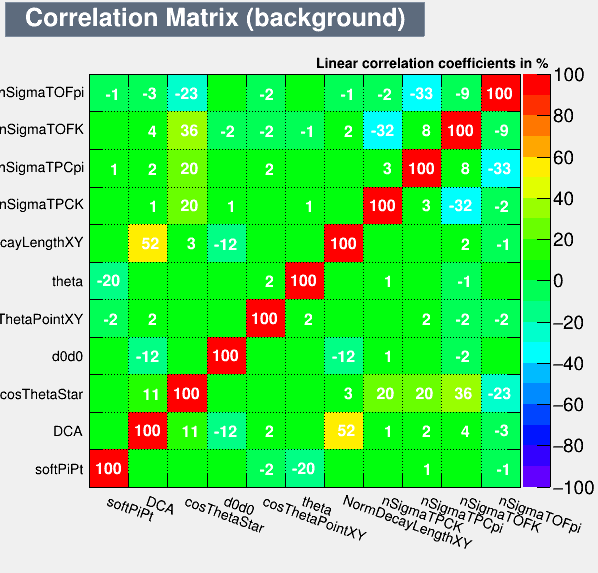
\includegraphics[width=7.5cm]{training&testing/CorrelationMatrixB.png}
        \captionof{figure}{Correlazione lineare in percentuale tra le variabili di taglio considerate per il training finale del fondo (da simulazione Monte Carlo)}
        \label{fig:correlazFinaleB}
        \end{flushright}
    \end{minipage} \\[1.cm]
    
%        \begin{figure}[htbp] %grafico correlazione lineare variabili finali
%        \centering
%        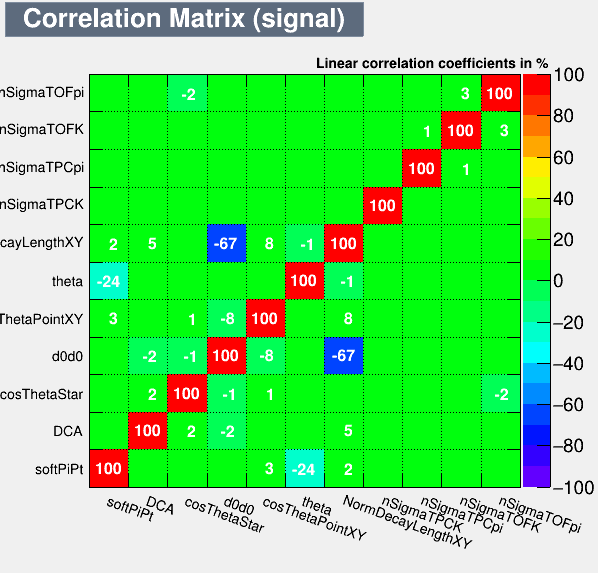
\includegraphics[width=0.7\linewidth]{training&testing/CorrelationMatrixS.png}
%        \caption{Correlazione lineare in percentuale tra le variabili di taglio considerate per il training finale del segnale (da simulazione Monte Carlo)}
%        \label{fig:correlazFinaleS}
%    \end{figure}
    
%    \begin{figure}[htbp] %grafico correlazione lineare variabili finali
%        \centering
%        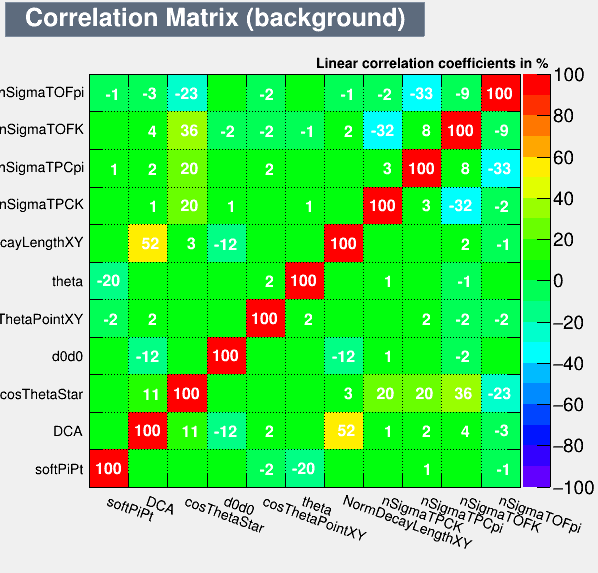
\includegraphics[width=0.7\linewidth]{training&testing/CorrelationMatrixB.png}
%        \caption{Correlazione lineare in percentuale tra le variabili di taglio considerate per il training finale del fondo (da simulazione Monte Carlo)}
%        \label{fig:correlazFinaleB}
%    \end{figure} 
    
    
  
  
\section{Training}

\subsection{Scelta dei dati per il training}
Come si è detto in precedenza per il training del BDT si sono utilizzati dati provenienti da \textit{simulazioni Monte Carlo}. Queste permettono, infatti, di simulare la collisione di fasci di protoni e le particelle che vengono create. I dati forniti dal Monte Carlo, però, non sono del tutto aderenti alla realtà fisica prodotta nell'esperimento di LHC, specialmente se si considera il fondo. 
\\ Inizialmente si sono utilizzati i dati delle simulazioni Monte Carlo ma per cercare di descrivere meglio il fondo si è, poi, deciso di considerare per la parte del \textit{segnale} i dati provenienti da simulazione Monte Carlo, mentre per il \textit{fondo} i dati dell'esperimento ALICE. È quindi necessario riuscire a selezionare dagli istogrammi dei dati di ALICE in funzione della diff${D^{*+}D^0}$ ( come il grafico \ref{fig:grafmassDstar1}) solamente il fondo senza prendere anche parte del segnale. Per fare questo si è scelto un valore minimo della variabile diff${D^{*+}D^0}$ e si sono presi solo i dati a destra di tale valore. Per scegliere il valore minimo si sono utilizzati sia il valore della massa del $\pi^+$ (che è la differenza tra la massa della $D^{*+}$ e della $D^0$), sia gli istogrammi dei dati di ALICE per alti intervalli di $p_T$ in cui il picco è più facilmente distinguibile \ref{fig:grafmassDstar1}, sia i primi risultati ottenuti dall'analisi che era stata già terminata utilizzando solo simulazioni Monte Carlo per il training e in cui era in parte distinguibile il picco del segnale anche per $p_T$ più bassi. Il valore scelto come limite inferiore è di $147.8 \ MeV/c^2$, che evidentemente più alto della massa del $\pi^+$ $139.5 \ MeV/c^2$.
\\A questo punto non c'erano più dati per il training che descrivessero il fondo a sinistra del picco, infatti in questo intervallo della diff${D^{*+}D^0}$ non è possibile individuare i dati corrispondenti solo al fondo e non al segnale come fatto prima. L'analisi dei dati di ALICE  ottenuta in questo modo, non distingueva bene il segnale dal fondo nella parte sinistra del picco, evidenziando la difficoltà dell'algoritmo nel selezionare le $D^{*+}$ in assenza di dati per il training in un particolare intervallo. 
\\Per risolvere questo problema si è deciso di utilizzare i dati della simulazione Monte Carlo per il fondo a sinistra del picco del segnale. I dati del fondo della simulzione Monte Carlo, pur non descrivendo al meglio i dati reali di ALICE, hanno fornito comunque una base per il training del BDT nella parte a sinistra del picco del segnale ed hanno permesso di ottenere risultati migliori nel riconoscimento delle $D^{*+}$. 
\\In figura \ref{fig:dati_training} è riportato il grafico dei dati utilizzati per il training per l'intervallo di $p_T$ [3-4]. Si vede in blu il segnale generato con simulazione Monte Carlo, in rosso il fondo a sinistra generato con simulazione Monte Carlo e in verde il fondo a destra preso dai dati di ALICE. Come si nota in \ref{fig:dati_training} i dati del fondo a destra non ci sono per valori alti della diff${D^{*+}D^0}$, questo semplicemente perchè l'analisi per distinguere segnale da fondo è rivelante solo nell'intorno del piccodi segnale, mentre dove mancano i dati per il training siamo già sicuri sia solo fondo. 


    \begin{figure}[htbp] 
        \centering
        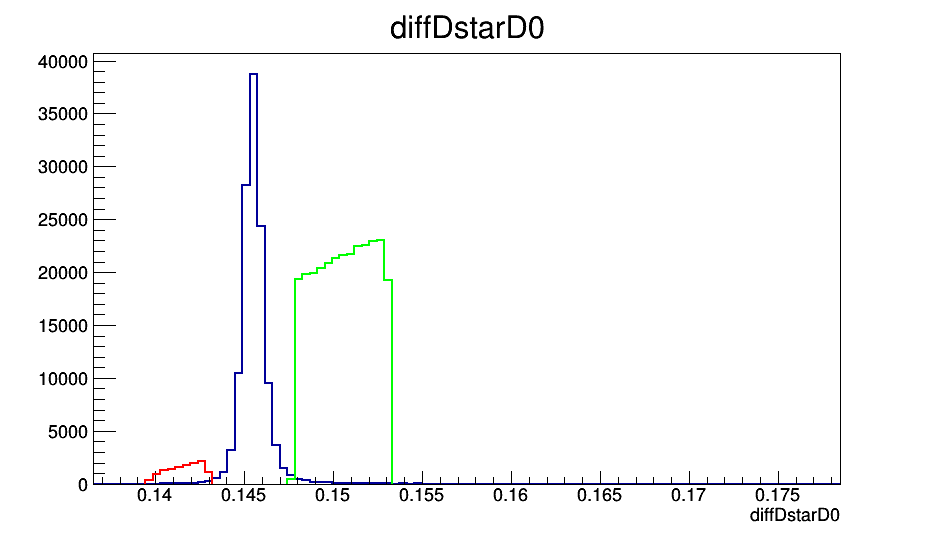
\includegraphics[width=0.9\linewidth]{training&testing/diffDstarD0_training_3_4_ok.png}
        \caption{Dati utilizzati per il training per l'intervallo di $p_T$ [3-4]: in blu il segnale, in rosso il fondo a sinistra ed in verde il fondo a destra }
        \label{fig:dati_training}
    \end{figure}
    
    
    

\subsection{Scelta dei Parametri del BDT}
L'algoritmo del BDT ha al suo interno alcuni parametri che possono essere variati e che possono cambiare l'efficienza dell'algoritmo stesso nel risolvere il problema. Per l'analisi svolta in questa tesi sono stati considerati nello specifico solo due parametri. Il primo è il \textit{numero di alberi} che compongono la "foresta" del BDT. Come spiegato nel paragrafo \ref{BDT}  il training vene fatto su un grande numero di alberi il cui responso viene unito in un'unica variabile finale. Aumentando il numero di alberi l'efficienza dell'algoritmo migliora, finché non si raggiunge un plateau e i risultati dell'analisi non variano all'aumentare del numero di alberi. Dato che un maggiore numero di alberi della foresta significa maggiore tempo impiegato sia per il training che per l'analisi dei dati, si è cercato il numero minimo di alberi che restituisse i risultati migliori ottenibili.
\\Il numero standard di alberi della foresta è di 850, ma variando questo numero si è trovato che già per 300 alberi i risultati erano gli stessi. Pertanto nell'analisi finale, di cui si riporteranno i risultati nel capitolo seguente, l'algoritmo del BDT ha 300 alberi. 
\\Il secondo parametro considerato è la \textit{profondità massima} di ogni albero. Con profondità si intende il numero di livelli di un albero. Ad esempio, in figura \ref{fig:depthBDT} l'albero ha 3 livelli, perchè per arrivare dal nodo principale all'ultima foglia ci sono 3 diverse diramazioni.
\\
    \begin{figure}[htbp] 
        \centering
        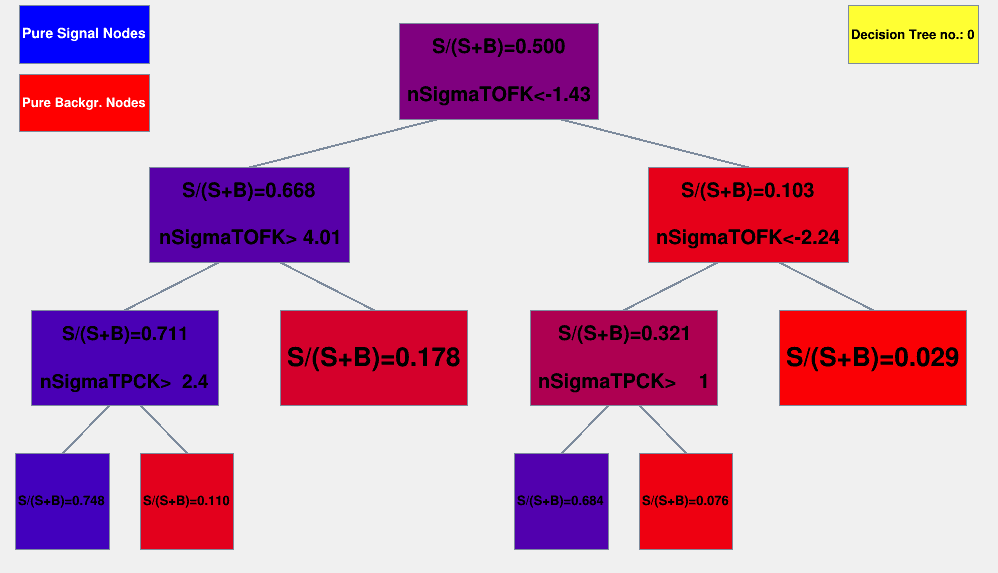
\includegraphics[width=0.7\linewidth]{training&testing/depthBDT.png}
        \caption{Schema di un albero del BDT con 3 livelli}
        \label{fig:depthBDT}
    \end{figure}
    
In questo caso si è visto che diminuendo la profondità massima a 2 livelli le performance dell'algoritmo peggiorano, mentre non c'è guadagno nell'aumentarla a 4. Dato che aumentando il numero massimo di livelli aumenta il tempo necessario per il training, l'analisi finale dei dati di ALICE è stata svolta con il parametro della profondità massima uguale a 3.

\subsection{I risultati del Training}

Alla fine del training della foresta di alberi,le caratteristiche di ogni albero, quindi i nodi di cui è composto, le variabili su cui si è discriminato, l'identificazione delle foglie come segnale o fondo, i pesi dei vari rami, vengono salvate in automatico. Questi valori vengono poi utilizzati per l'analisi dei dati di ALICE. 
\\Per valutare le performance dell'algoritmo del BDT utilizzato si possono considerare alcune grandezze, la prima è la \textit{ROC-Curve} (Receiving Operating Characteristics Curve) e in particolare l'area sottesa alla ROC-Curve. La ROC-Curve è il grafico della background rejection in funzione della signal efficiency. Dove la background rejection è 1 - background efficiency, la background efficiency è il numero di eventi del fondo selezionati come fondo e la signal efficiency è il numero di eventi segnale selezionati come segnale.
Un algoritmo è tanto più efficiente quanto più è alto il valore dell'area della Roc-Curve. %, il cui  limite teorico è fissato dal Likelihood Ratio.
Riportiamo in figura \ref{fig:RocCurve} il grafico della ROC-Curve relativa al training del bin di $p_T$ [3-4] con 300 alberi con profondità massima 3, che è stato utilizzato poi per l'analisi dei dati. In questo caso l'area sottesa alla curva è ROC-integral = 0.945 . 
    \begin{figure}[htbp] 
        \centering
        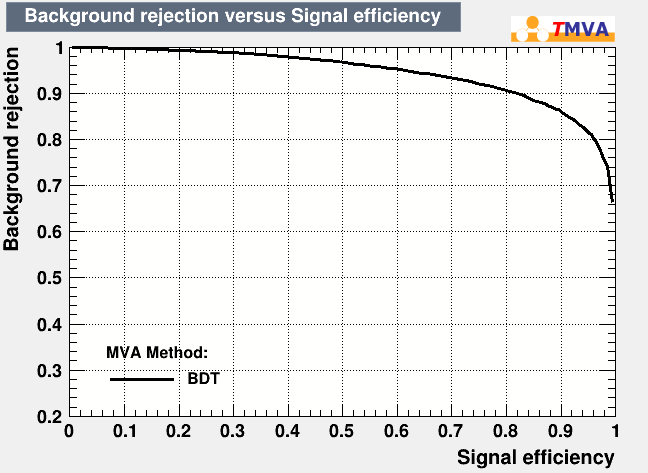
\includegraphics[width=0.7\linewidth]{training&testing/RocCurve.png}
        \caption{Grafico della ROC-Curve relativa al training del BDT con 300 alberi e profondità massima 3}
        \label{fig:RocCurve}
    \end{figure}
    
Un'altra grandezza da considerare è la distribuzione dei dati in funzione del classifier output (di cui si è parlato nel \ref{AnalisiMulti}), che in questo caso è chiamato \textit{BDTresponse}. Questo ci da una prima indicazione di quanto sarà possibile separare il segnale dal fondo, infatti, laddove si sovrappongono non sarà possibile separare segnale e fondo quando si utilizzerà questo BDT sui dati di ALICE. Il grafico in figura \ref{fig:BDTresponse} mostra proprio la distribuzione dei dati del testing in funzione del BDTresponse. Si utilizzano i dati del testing proprio per fare dei test sulle performance dell'algoritmo. 

    \begin{figure}[htbp] 
        \centering
        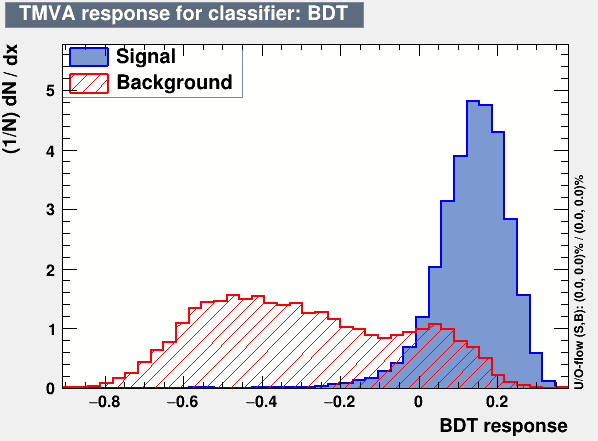
\includegraphics[width=0.7\linewidth]{training&testing/BDTresponsetest.png}
        \caption{Distribuzione dei dati del testing rispetto al BDTresponse del training con 300 alberi e profondità massima 3}
        \label{fig:BDTresponse}
    \end{figure}
    
Se confrontiamo la distribuzione dei dati in figura \ref{fig:BDTresponse} e quella rispetto alle variabili di taglio in figura \ref{fig:variabilitaglio}, si nota facilmente quanto la differenza tra la distribuzione del fondo e del segnale sia aumentata considerando il BDTresponse, piuttosto che le grandezze fisiche delle variabili di taglio. Questo è proprio il vantaggio offerto dall'analisi multivariata e in nel caso specifico dall'algoritmo del BDT.
    
\\Infine è importante anche considerare l'\textit{efficienza del BDT}, che come detto in precedenza è il numero degli eventi segnale che sono stati classificati come segnale dall'algoritmo. Pertanto se l'efficienza è 1 tutti gli eventi segnale sono stati riconosciuti come tali, mentre se è 0 tutti gli eventi segnale sono stati classificati come fondo. Si deve notare, però, che anche nel caso in cui  l'efficienza sia 1 è possibile (anzi probabile) che alcuni eventi fondo siano stati classificati come segnale e perciò la selezione ha comunque dei problemi.
\\Per questo motivo si considerano anche altre grandezze quali l'efficienza del fondo e la significatività, quest'ultima è definita come 

    \begin{equation}
        s \ = \ \frac{eff_{segnale}}{\sqrt{eff_{segnale} + eff_{fondo}}}
    \end{equation}{}

Sia l'efficienza del segnale, che l'efficienza del fondo, che la significatività variano in base al valore del taglio applicato al valore del BDTresponse. Il taglio è il valore scelto come limite per dividere il segnale dal fondo, per esempio, considerando il grafico di figura \ref{fig:BDTresponse}, più il valore del taglio è alto più l'efficienza del segnale aumenta ma l'efficienza del fondo diminuisce. Si riporta in figura \ref{fig:effBDT} il grafico di queste grandezze al variare del valore del taglio, per il training fatto con 300 alberi e profondità massima 3.
\\

    \begin{figure}[htbp] 
        \centering
        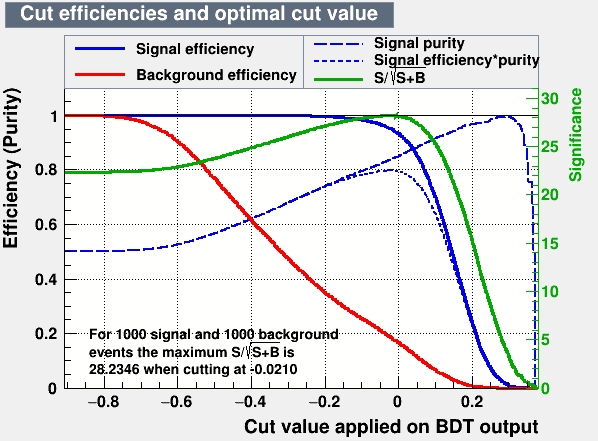
\includegraphics[width=0.7\linewidth]{training&testing/effBDT.png}
        \caption{Grafico dell'efficienza del segnale in blu, efficienza del fondo in rosso e significatività in verde, al variare del valore del taglio scelto per la BDTresponse. Gli andamenti sono relativi al training con 300 alberi e profondità massima 3}
        \label{fig:effBDT}
    \end{figure}
    
Attraverso le grandezze di cui si è appena parlato è quindi stato possibile fare delle verifiche sulle performance e sull'utilità dell'algoritmo del BDT per l'analisi dati che si vuole svolgere in questa tesi. In particolare si sono notati due problemi principali utilizzando il BDT. Da un lato considerando l'intervvalo di $p_T$ [1,2], ovvero il più basso considerato in questa analisi, si sono subito riscontrati dei problemi. Già i risultati del training, infatti, sono solo parziali. In particolare il problema sta nel numero molto basso di eventi segnale nei dati della simulazione Monte Carlo. Ricordiamo, infatti, che a basso $p_T$ ci sono molti più eventi fondo rispetto al segnale, ma per il bin di $p_T$ che stiamo considerando gli eventi segnale appartenenti al dataset della simulazione usata per il training è molto basso, nel caso specifico si hanno appena $117$ eventi segnale (contro i circa $100000$ del fondo). 
\\A questo punto è fondamentale ricordare che i metodi di analisi basati sul Machine Learning funzionano bene quando si utilizzano grandi quantità di dati, infatti è proprio grazie ai numerosi esempi su cui viene fatto il training che l'algoritmo impara a riconoscere e selezionare le varie tipologie di dati. 
È quindi evidente il problema di utilizzare per il training solamente $90$ eventi per il segnale. In questo caso si è considerato circa l'$80\%$ dei 117 eventi totali per il training e il restante $20\%$ per il testing. Si riporta il grafico della distribuzione dei dati in funzione del BDTresponse. 

 \begin{figure}[htbp] 
        \centering
        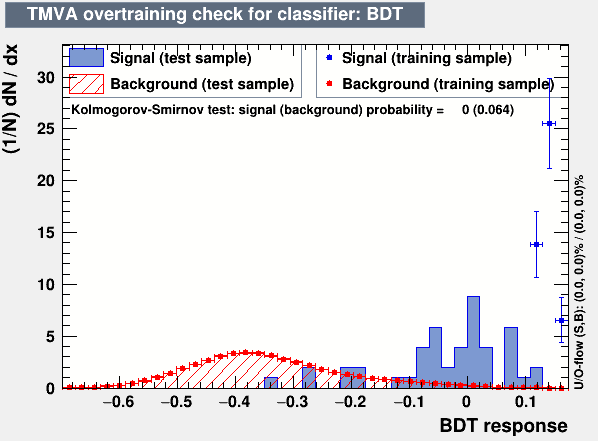
\includegraphics[width=0.7\linewidth]{training&testing/BDTresponse_0_1.png}
        \caption{Distribuzione dei dati di training e testing rispetto al BDTresponse del training con 300 alberi e profondità massima 3 per il bin di $p_T$ [0,1]. I rettangoli rappresentano i risultati del testing, i punti con i relativi errori i risultati del training.
        }
        \label{fig:BDTresponse_0_1}
    \end{figure}
    
Come si vede dal grafico \ref{fig:BDTresponse_0_1} la distribuzione dei dati del segnale del testing non è uniforme ed è molto sovrapposta a quella del fondo, questo rende difficile individuare un buon valore del taglio della BDTresponse e in generale poco efficace il metodo del BDT per la selezione delle $D^*+$. Inoltre si nota anche che le distribuzioni dei dati del training e del testing del segnale differiscono notevolmente fra loro. Come verrà spiegato più avanti nella sezione \ref{testing}, questo è un altro indice che iil BDT non sta funzionando correttamente. Per questi motivi si è deciso di non continuare l'analisi per il bin di $p_T$ [0,1] ma solo per $p_T \ > 1 \  Gev/c$. 
\\Il secondo problema con l'utilizzo del BDT si è riscontrato per i bin di $p_T$ più alto, ovvero [12,16] e [16,24].  Il problema anche in questo caso sta nel numero troppo basso di eventi, ovvero la statistica è troppo poca per permettere al BDT di funzionare correttamente. Inoltre, si deve considerare che all'aumentare del $p_T$ il picco di segnale nella distribuzione dei dati di ALICE rispetto alla variabile $diffD^{*+}D^0$ diventa sempre più evidente e più facilmente individuabile anche con un'analisi che non utilizza metodi multivariati. 

%___________RIVEDERE ALTO PT________________________________-
%_________________________________________________
%___________________________________________________



\subsection{Scelta dei valori di taglio}

L'ultima operazione da compiere per concludere il training del BDT è quella di scegliere i valori di taglio della variabile BDTresponse, che permettono poi nella fase di analisi dei dati di ALICE di discriminare tra segnale e fondo. Per scegliere i valori di taglio si è fatto riferimento da una parte ai grafici delle efficienze e della significatività di cui si è parlato precedentemente, dall'altra si sono confrontati i risultati dell'analisi dei dati di ALICE (di cui si parla nel capitolo \ref{Analisi} e come questi variano in base al taglio. 

Nell'utilizzare i grafici di efficienze e significatività per la scelta del valore di taglio è stato fondamentale aver considerato un rapporto segnale-fondo molto basso (10:1000), questo perchè nei dati di ALICE abbiamo che gli eventi segnale sono molti meno degli eventi fondo. In tal modo anche i risultati del training del BDT e le curve di efficienze e significatività sono più aderenti ai dati di ALICE su cui si svolge in seguito l'analisi. 

    \begin{figure}[htbp] 
        \centering
        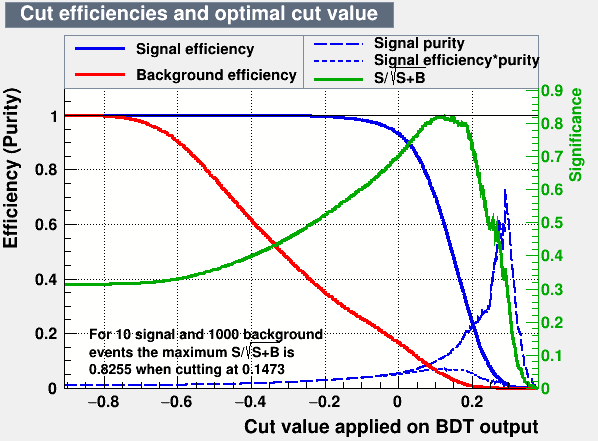
\includegraphics[width=0.7\linewidth]{training&testing/effBDT/effBDT_rapp_3_4.png}
        \caption{Grafico dell'efficienza del segnale in blu, efficienza del fondo in rosso e significatività in verde, al variare del valore del taglio scelto per la BDTresponse per il bin di $p_T$ [3,4]. Il rapporto tra segnale e fondo è di 10:1000 . Gli andamenti sono relativi al training con 300 alberi e profondità massima 3
        }
        \label{fig:effBDT_10_1000}
    \end{figure}
    
Una scelta per il valore di taglio inizialmente presa in considerazione è il punto di massimo della significatività. L'analisi dei dati di ALICE. però, è stata svolta anche per altri valori di taglio del BDTresponse è si è visto che abbassando di poco il valore di taglio la significatività dei dati di ALICE aumentava. In particolare si è scelto il punto in cui la curva dell'efficienza del segnale e quella della significatività si incontrano, cercando così di avere un buon compromesso tra la quantità di segnale selezionata e la significatività. Per i bin di $p_T$ più alti i grafici della significatività diventano sempre meno lineari. probabilmente a causa del diminuire della quantità di dati utilizzata per il training, pertanto in alcuni casi è stato scelto un valore di taglio più alto rispetto a quello del metodo precedentemente indicato. 
In tabella \ref{valori_taglio} si riportano i valori di taglio della BDTresponse per tutti gli intervalli di $p_T$ su cui è stata svolta l'analisi finale.

    \begin{table}[H]
		\centering
		\begin{tabular}{c|c}
		    \toprule
		    bin $p_T$   &   valore del taglio  \\
            \midrule
            1 - 2  	&    0.049   \\ 
            2 - 3 	&    0.045  \\ 
            3 - 4  	&    0.031  \\ 
            4 - 5  	&    0.027  \\ 
            5 - 6  	&    0.031  \\ 
            6 - 8  	&    0.034  \\ 
            8 - 12  &    0.105  \\   
			\bottomrule
			\label{valori_taglio}
		\end{tabular}
	\end{table}
    
 
 
 
 
 \section{Testing}
 
 Come si è già detto in precedenza, una oarte dei dati generati dalla simulazione Monte Carlo non viene utilizzata per il training, ma è lasciata per la fase di testing. Si vuole controllare, in particolare che non ci sia stato overtraining e perciò ci si aspetta che la distribuzione dei dati al variare del valore della BDTresponse sia la stessa. Riportiamo ora alcuni grafici esemplificativi del controllo per l'overtraining per alcuni bin di $p_T$.
 
 
    \begin{minipage}{.5\textwidth}%{0.5 cm} 
        \begin{flushleft} \large
        \flushleft
        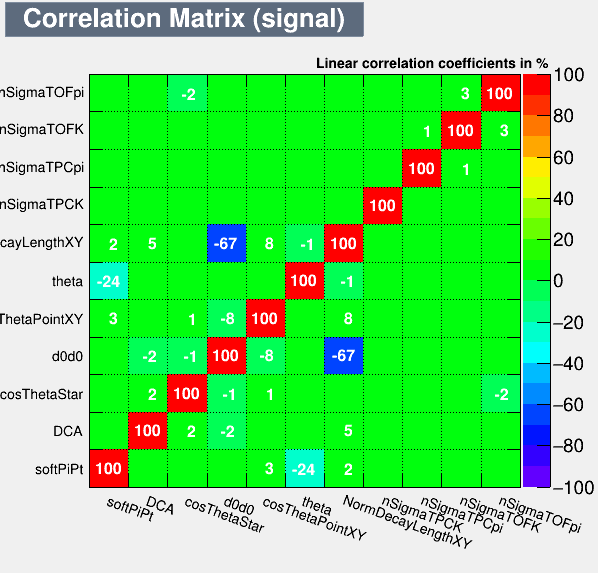
\includegraphics[width=7.5cm]{training&testing/CorrelationMatrixS.png}
        \captionof{figure}{Distribuzione dei dati del training (con i punti e relativi errori) e del testing (con i rettangoli) al variare della BDTresponse per il bin di $p_T$ [3,4]}
        \label{fig:testing_3_4}
        \end{flushleft}
        \end{minipage}
    ~
    \begin{minipage}{0.5\textwidth}
        \begin{flushright} \large
        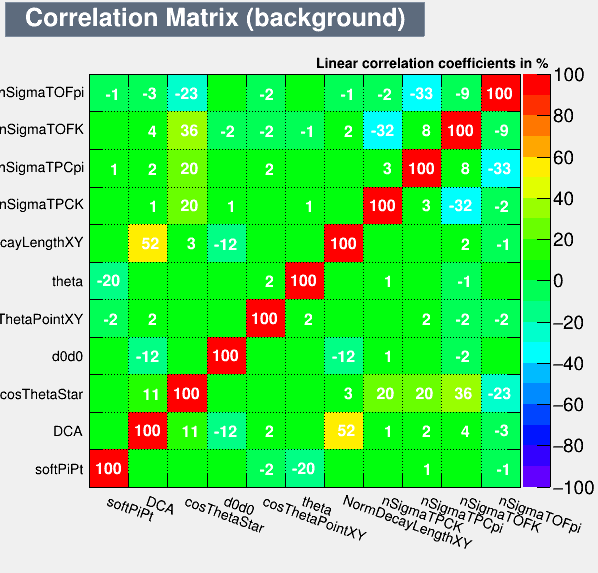
\includegraphics[width=7.5cm]{training&testing/CorrelationMatrixB.png}
        \captionof{figure}{Distribuzione dei dati del training (con i punti e relativi errori) e del testing (con i rettangoli) al variare della BDTresponse per il bin di $p_T$ [6,8]}
        \label{fig:testing_6_8}
        \end{flushright}
    \end{minipage} \\[1.cm]
    
Come si vede dai grafici \ref{fig:testing_3_4} e \ref{fig:testing_6_8}. le distribuzioni dei dati per il training e il testing coincidono.
\chapter{Analisi dei dati di ALICE} \label{Analisi}


\section{I Dati Iniziali}

I dati utilizzati per l'analisi svolta sono relativi a collisioni di due fasci di protoni incidenti al Cern. I dati, racccolti nel 2017 da ALICE, sono caratterizzati da un valore di energia nel centro di massa di 5 \ $TeV$. 
\\Da questi dati si vogliono selezionare solo le $D^{*+}$, che sono state ricostruite dal decadimento $D^{*+} \rightarrow D^0 + \pi^+ $. Per fare ciò, ai dati utilizzati sono già state applicate delle pre-selezioni estremamente morbide che permettono di preservare tutto il segnale e di fare una prima scrematura dei dati grezzi.
Gli intervalli di $p_T$ considerati sono: [1,2], [2,3], [3,4], [4,5], [5,6], [6,8], [8,12] misurati in GeV/c. 
La distribuzione di massa invariante iniziale, cioè prima dell'applicazione del BDT, è visibile in figura \ref{fig:grafmassDstar1} per l'intervallo di $p_T$ [2,3] $GeV/c$.

    \begin{figure}[htbp]
        \centering
        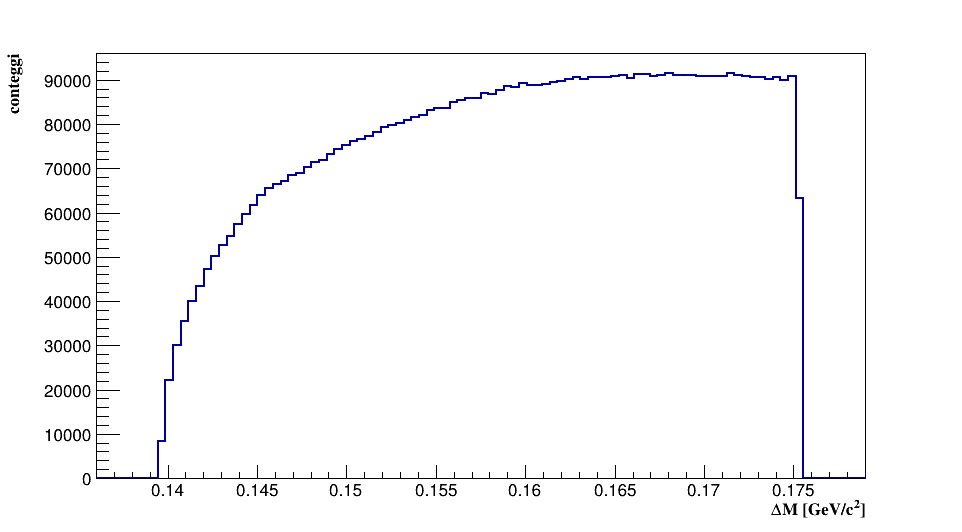
\includegraphics[width=0.7\linewidth]{AnalisiDati/dati_2_3.png}
        \caption{Distribuzione della differenza di massa invariante tra la $D^{*+}$ e la $D^0$, $\Delta M = M(\pi^+,\pi^+,K^-) - M(\pi^+,K^-)$, per l'intervallo di $p_T$ [2,3] $GeV/c$}
        \label{fig:grafmassDstar1}
    \end{figure}
    
Nel grafico \ref{fig:grafmassDstar1} non si vede nessun picco evidente, cosa che ci si aspetta nel caso di una risonanza come la $D^{*+}$. Questo accade perché il numero di $D^{*+}$ prodotte è troppo piccolo rispetto al fondo combinatoriale delle combinazioni di particelle non relative alla $D^{*+}$ e pertanto il picco della $D^{*+}$ non è riconoscibile rispetto al fondo.

    \begin{figure}[htbp]
        \centering
        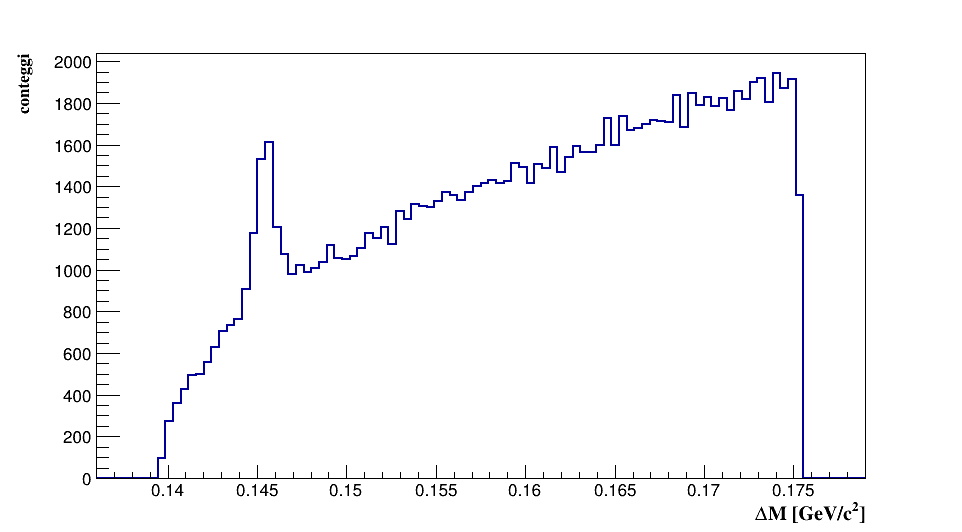
\includegraphics[width=0.7\linewidth]{AnalisiDati/dati_6_8.png}
        \caption{Distribuzione della differenza di massa invariante tra la $D^{*+}$ e la $D^0$, $\Delta M = M(\pi^+,\pi^+,K^-) - M(\pi^+,K^-)$, per l'intervallo di $p_T$ [6,8] GeV/c}
        \label{fig:grafmassDstar2}
    \end{figure}

Nel grafico della distribuzione di massa invariante \ref{fig:grafmassDstar2} in cui si considera l'intervallo di $p_T$ [6,8] GeV/c il picco della $D^{*+}$ è visibile e riconoscibile rispetto al fondo. 
\\In generale all'aumentare del valore del $p_T$ diventa più evidente il picco di segnale nelle distribuzioni di massa invariante. Questo accade perché nelle collisioni pp vengono prodotti più $\pi^+$ e $K^-$ con basso $p_T$ che con alto $p_T$ e perciò anche il fondo combinatoriale è maggiore a basso $p_T$.


\section{Applicazione del BDT}
Una volta finite le fasi di training e testing si può procedere all'applicazione del BDT sui dati che si vogliono analizzare. La struttura del BDT creata nella fase di training e  controllata nella fase del testing viene ora utilizzata per discriminare i dati tra segnale e fondo. Pertanto il BDT con 300 alberi, profondità massima 3 e con i valori di taglio indicati nella tabella \ref{Tab:tagli} è stato applicato per ogni intervallo di $p_T$ considerato, ottenendo così una selezione dei dati.
\\In figura \ref{fig:diffDstarD0_3_4_BDT} è riportata la distribuzione in massa invariante delle candidate $D^{*+}$ selezionate con il metodo BDT. Si vede il picco del segnale evidente attorno al valore della $ \Delta M = M(\pi^+,\pi^+,K^-) - M(\pi^+,K^-) \ \simeq \ 0.145 \ GeV/c$, sovrapposto ad un fondo residuo.


 \begin{figure}[htbp] 
        \centering
        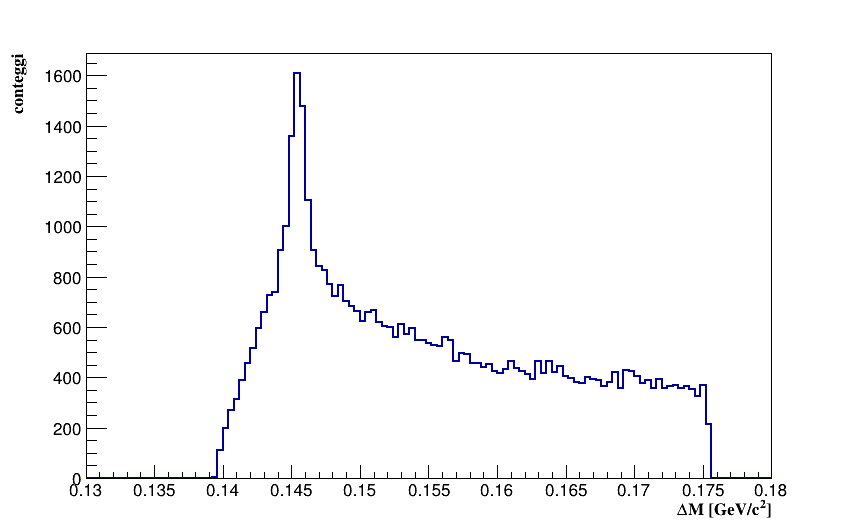
\includegraphics[width=0.7\linewidth]{AnalisiDati/diffDstarD0_3_4BDT.png}
        \caption{Distribuzione di massa invariante $\Delta M = M(\pi^+,\pi^+,K^-) - M(\pi^+,K^-)$, per l'intervallo di $p_T$ [3,4] GeV/c}
        \label{fig:diffDstarD0_3_4_BDT}
    \end{figure}
    
Per determinare il numero di candidate $D^{*+}$ selezionate si è proceduto con il fit della distribuzione di massa invariante. 
\\Per l'intervallo di $p_T$ [1-2] $GeV/c$ i dati della distribuzione di massa invariante delle candidate $D^{*+}$ selezionate con il metodo BDT non mostra un picco di segnale. Per questo motivo si è deciso di non procedere con il fit della distribuzione per questo intervallo di $p_T$ e perciò i risultati seguenti vengono mostrati solo per $p_T > 2 \ GeV/c$.
\\Per gli intervalli di $p-T$ considerati il picco del segnale é stato descritto da una funzione Gaussiana, mentre il fondo é stato descritto dalla somma di due funzioni:

    \begin{equation}
        fondo_1  = \ d \sqrt{x-0.13957} e^{- (x - 0.13857) }
    \end{equation}
     \begin{equation}
        fondo_2 = \ a x^2 + b x + c
    \end{equation}
    
Dove $a, \ b, \ c, e d$ sono dei parametri liberi utilizzati per il fit del fondo.
\\La $Gaussiana$ ha come range [0.144,0.147] , la funzione $fondo_1$ [0.1395,0.155] e $fondo_2$  [0.1435,0.150]. Le due funzioni per il fondo vengono prima sommate e poi la nuova funzione $fondo$ = $fondo_1$ + $fondo_2$ viene fatto il fit nell'intervallo [0.1395,0.1545]. Infine si sommano le funzione $fondo$ e $Gaussiana$ ottenendo la funzione chiamata $totale$, da cui il fit finale mostrato in figura \ref{fig:fit_3_4}.

    \begin{figure}[htbp] 
        \centering
        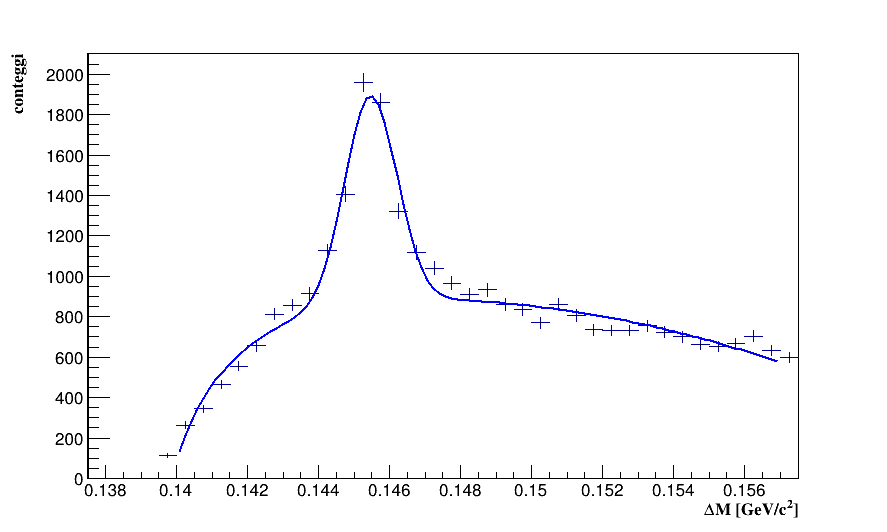
\includegraphics[width=0.9\linewidth]{AnalisiDati/pt_3_4_pol2.png}
        \caption{Distribuzione di massa invariante $\Delta M = M(\pi^+,\pi^+,K^-) - M(\pi^+,K^-)$, per l'intervallo di $p_T$ [3,4] GeV/c e funzione di fit $totale$ in blu}
        \label{fig:fit_3_4}
    \end{figure}
    
Si nota che all'aumentare del $p_T$ il fondo diminuisce sempre di più e tende ad appiattirsi, rendendo così il fit più semplice.
Si riportano di seguito i grafici per i vari bin di $p_T$ considerati. 
\\

\begin{minipage}{.5\textwidth}%{0.5 cm} 
        \begin{flushleft} \large
        \flushleft
        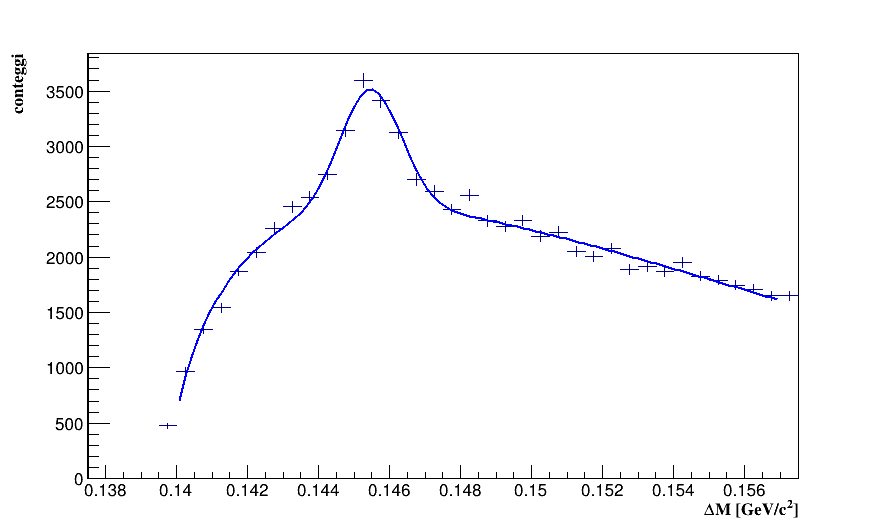
\includegraphics[width=8cm]{AnalisiDati/pt_2_3_pol2.png}
        \captionof{figure}{Distribuzione di massa invariante $\Delta M = M(\pi^+,\pi^+,K^-) - M(\pi^+,K^-)$, per l'intervallo di $p_T$ [2,3] GeV/c e funzione di fit $totale$ in blu}
        \label{fig:fit_2_3}
        \end{flushleft}
        \end{minipage}
    ~
    \begin{minipage}{0.5\textwidth}
        \begin{flushright} \large
        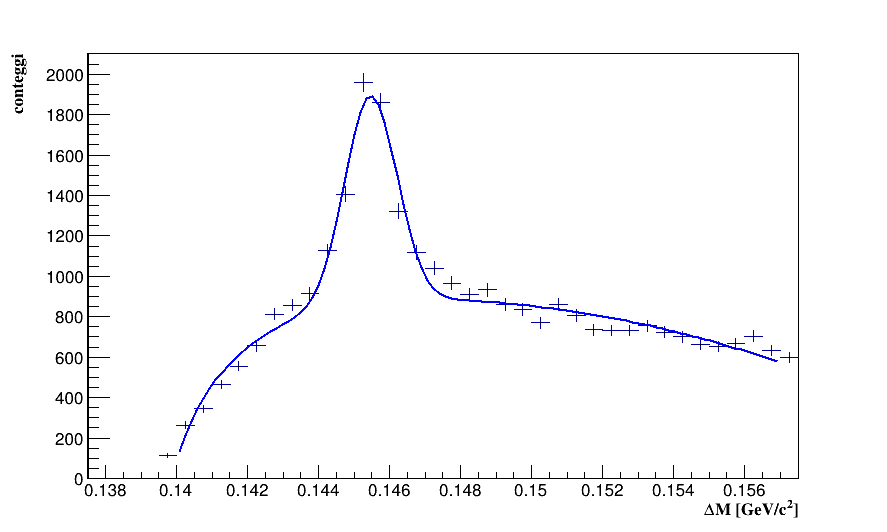
\includegraphics[width=8cm]{AnalisiDati/pt_3_4_pol2.png}
        \captionof{figure}{Distribuzione di massa invariante $\Delta M = M(\pi^+,\pi^+,K^-) - M(\pi^+,K^-)$, per l'intervallo di $p_T$ [3,4] GeV/c e funzione di fit $totale$ in blu}
        \label{fig:fit_3_4_p}
        \end{flushright}
    \end{minipage} \\[1.cm]
    
    
    \begin{minipage}{.5\textwidth}%{0.5 cm} 
        \begin{flushleft} \large
        \flushleft
        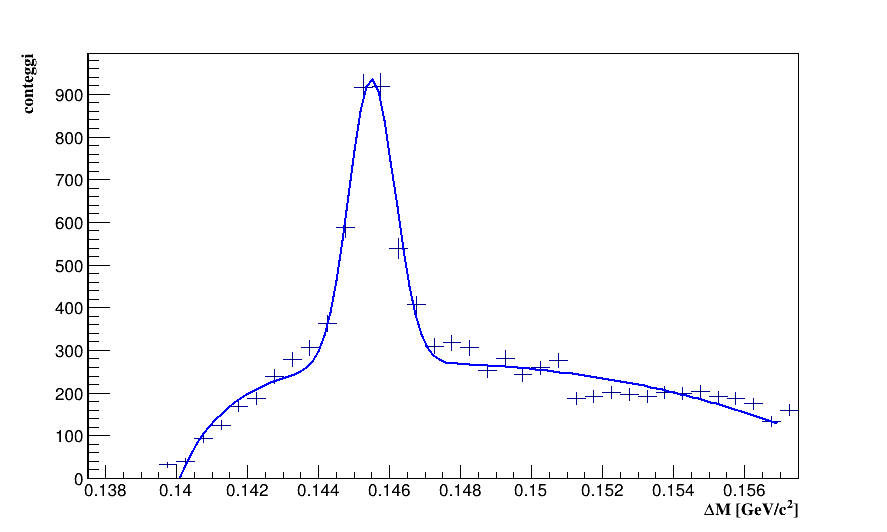
\includegraphics[width=8cm]{AnalisiDati/pt_4_5_pol2.png}
        \captionof{figure}{Distribuzione di massa invariante $\Delta M = M(\pi^+,\pi^+,K^-) - M(\pi^+,K^-)$, per l'intervallo di $p_T$ [4,5] GeV/c e funzione di fit $totale$ in blu}
        \label{fig:fit_4_5}
        \end{flushleft}
        \end{minipage}
    ~
    \begin{minipage}{0.5\textwidth}
        \begin{flushright} \large
        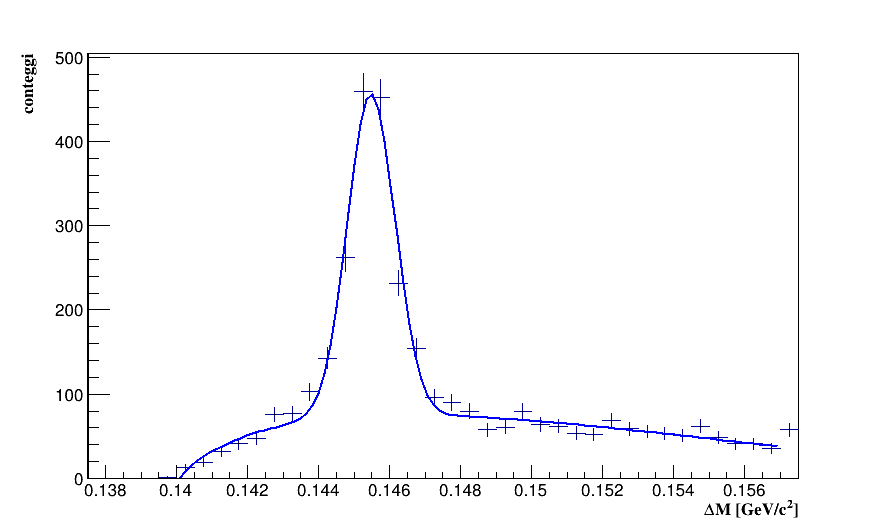
\includegraphics[width=8cm]{AnalisiDati/pt_5_6_pol2.png}
        \captionof{figure}{Distribuzione di massa invariante $\Delta M = M(\pi^+,\pi^+,K^-) - M(\pi^+,K^-)$, per l'intervallo di $p_T$ [5,6] GeV/c e funzione di fit $totale$ in blu}
        \label{fig:fit_5_6}
        \end{flushright}
    \end{minipage} \\[1.cm]

\begin{minipage}{.5\textwidth}%{0.5 cm} 
        \begin{flushleft} \large
        \flushleft
        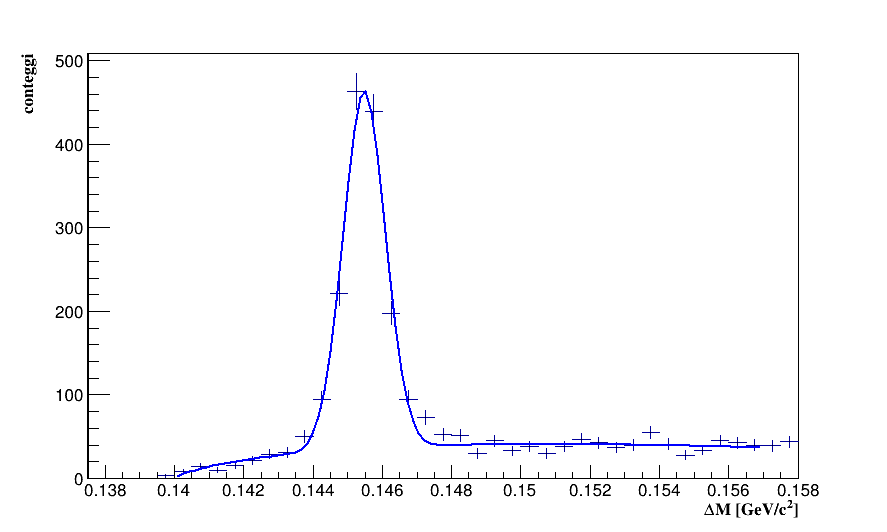
\includegraphics[width=8cm]{AnalisiDati/pt_6_8_pol2.png}
        \captionof{figure}{Distribuzione di massa invariante $\Delta M = M(\pi^+,\pi^+,K^-) - M(\pi^+,K^-)$, per l'intervallo di $p_T$ [6,8] GeV/c e funzione di fit $totale$ in blu}
        \label{fig:fit_6_8}
        \end{flushleft}
        \end{minipage}
    ~
    \begin{minipage}{0.5\textwidth}
        \begin{flushright} \large
        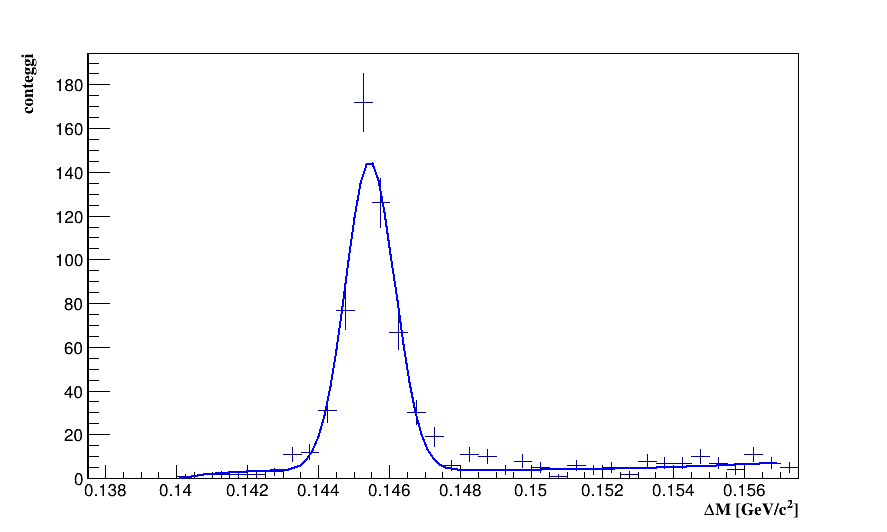
\includegraphics[width=8cm]{AnalisiDati/pt_8_12_pol2.png}
        \captionof{figure}{Distribuzione di massa invariante $\Delta M = M(\pi^+,\pi^+,K^-) - M(\pi^+,K^-)$, per l'intervallo di $p_T$ [8,12] GeV/c e funzione di fit $totale$ in blu}
        \label{fig:fit_8_12}
        \end{flushright}
    \end{minipage} \\[1.cm]
    


\section{Valutazione delle performance}

Per valutare le performance dell'analisi svolta si sono calcolate alcune grandezze quali la quantità di segnale selezionata, la quantità di fondo selezionata, la significatività e il rapporto segnale su fondo. Per poter avere queste grandezze in ogni intervallo di $p_T$ si è calcolato l'integrale della funzione di fit $totale$ entro 3 $\sigma$ a destra e a sinistra del valore medio della Gaussiana. Sia il valore medio della Gaussiana che il valore della $\sigma$ sono stati presi dal fit della Gaussiana sul picco del segnale. Poi si è trovata la quantità di fondo calcolando l'integrale della funzione $fondo$ nello stesso intervallo. Infine, per trovare la quantità di segnale, si è sottratto all'integrale della funzione $totale$ l'integrale del fondo. 
\\In figura \ref{fig:segnale} si riporta la quantità di segnale per i vari intervalli di $p_T$ con l'errore associato. Dalla figura si vede che l'efficienza del segnale diminuisce all'aumentare del $p_T$.

    \begin{figure}[htbp] 
        \centering
        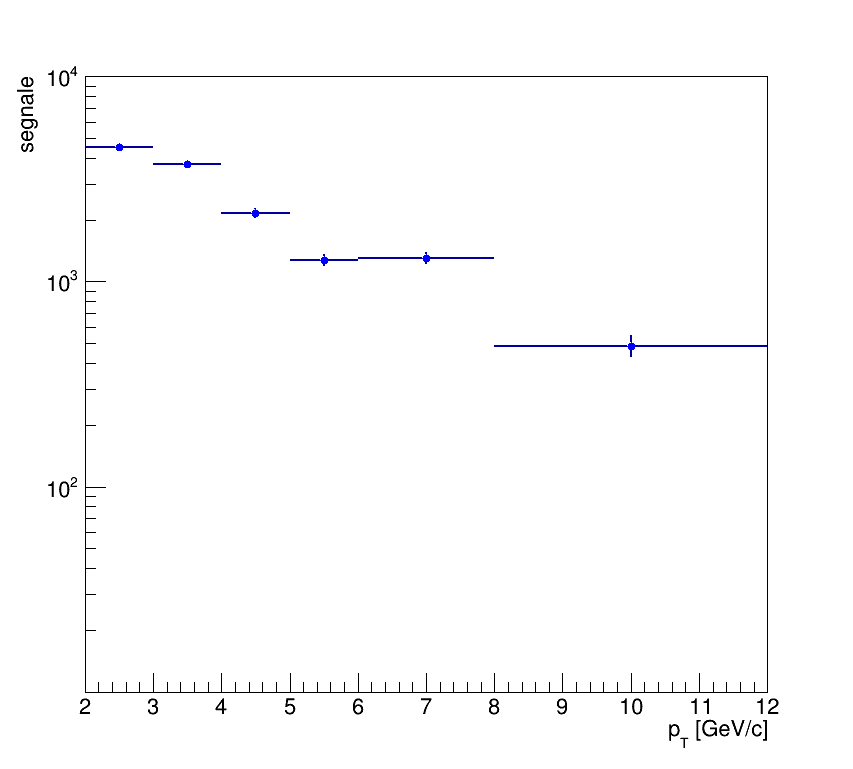
\includegraphics[width=0.9\linewidth]{AnalisiDati/segnale.png}
        \caption{Grafico della quantità di segnale in funzione del $p_T$}
        \label{fig:segnale}
    \end{figure}

In figura \ref{fig:fondo} è mostrata la quantità di fondo per gli intervalli di $p_T$ considerati. Si vede che l'efficienza del segnale diminuisce velocemente all'aumentare del $p_T$.

    \begin{figure}[htbp] 
        \centering
        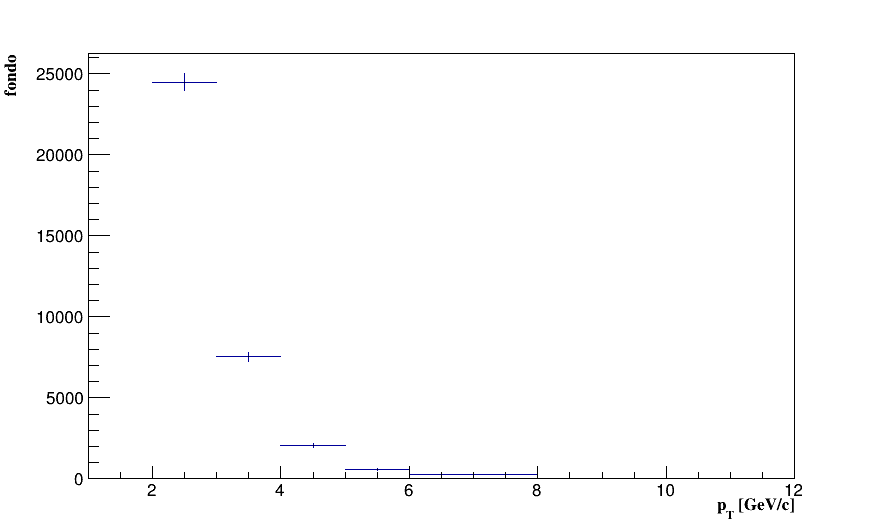
\includegraphics[width=0.9\linewidth]{AnalisiDati/fondo.png}
        \caption{Grafico della quantità di fondo in funzione del $p_T$}
        \label{fig:fondo}
    \end{figure}
    
Si è calcolata anche la significatività, utilizzando la formula 
 
 \begin{equation}
     sign = \frac{s}{\sqrt{s+f}}
 \end{equation}

dove $s$ è la quantità di segnale, mentre $f$ è la quantità di fondo. Anche in questo caso l'operazione è stata ripetuta per tutti gli intervalli di $p_T$ e con la propagazione degli errori si è ricavato l'errore relativo.

    \begin{figure}[htbp] 
        \centering
        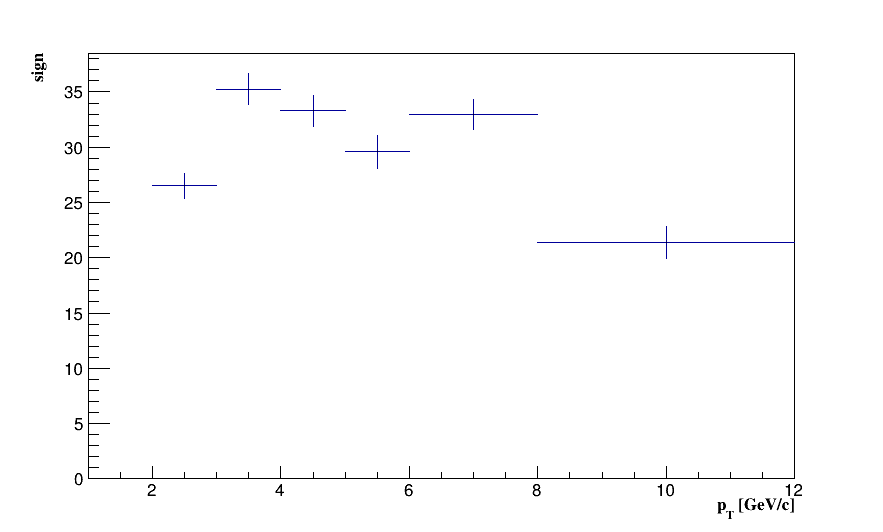
\includegraphics[width=0.9\linewidth]{AnalisiDati/significance.png}
        \caption{Grafico della significatività in funzione del $p_T$}
        \label{fig:significatività}
    \end{figure}

Il grafico in figura \ref{fig:significatività} mostra il valore della significatività per gli intervalli di $p_T$ considerati. Si vede che si ha il massimo della significatività per l'intervallo di $p_T$ [3,4] GeV/c e il minimo per l'intervallo di $p_T$ [8,12] GeV/c.
\\Si è creato anche il grafico del rapporto tra segnale e fondo al variare del bin di $p_T$ riportato in figura \ref{fig:s_b}. 

    \begin{figure}[htbp] 
        \centering
        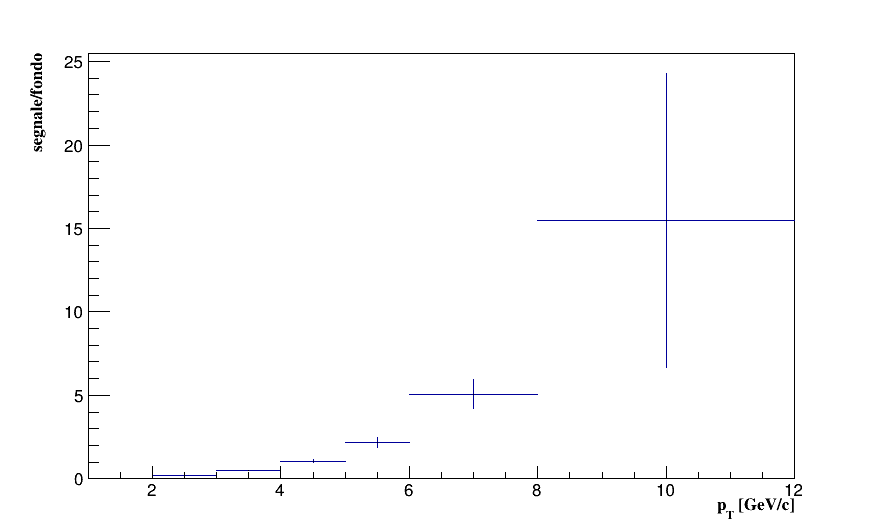
\includegraphics[width=0.9\linewidth]{AnalisiDati/s_b.png}
        \caption{Grafico del rapporto segnale su fondo in funzione del $p_T$}
        \label{fig:s_b}
    \end{figure}
    
Infine, in figura \ref{fig:confr_sign}, si confrontano i valori della significatività ottenuti con l'analisi del BDT e quelli ottenuti con l'analisi standard si ALICE. Si vede che per gli intervalli di $p_T < 4 \ GeV/c$ la significatività ottenuta con l'analisi del BDT è più alta di quella ottenuta con l'analisi standard di ALICE, mentre per $p_T > 4 \ GeV/c$ accade il contrario. 

\begin{figure}[htbp] 
        \centering
        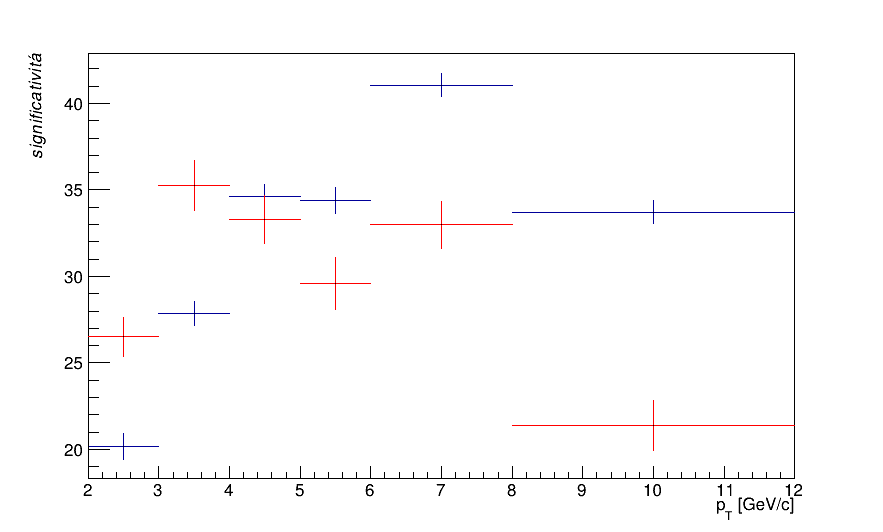
\includegraphics[width=0.9\linewidth]{AnalisiDati/confr_sign.png}
        \caption{Grafico della significatività in funzione del $p_T$, in blu l'analisi standard di ALICE, in rosso l'analisi con il BDT}
        \label{fig:confr_sign}
    \end{figure}

\chapter{Conclusioni}

In questa tesi sono stati analizzati i dati raccolti da ALICE in collisioni protone-protone ad LHC all'energia del centro di massa di 5~TeV e si è studiata la produzione del mesone $D^{*+}$ contenente un quark charm attraverso la ricostruzione del decadimento $D^{*+} \rightarrow D^{0}(\rightarrow \pi^+ K^-)\pi^+$. L'analisi è stata svolta utilizzando un algoritmo di analisi multivariata, il Boosted Decision Tree.

Il lavoro di questa tesi ha mostrato che \`e possibile utilizzare questi algoritmi per l'identificazione del mesone $D^{*+}$ e che l'utilizzo di questa tecnica risulta pi\`u utile quando si considerano candidate con un basso impulso trasverso ($p_T < 5 $~GeV/c) in quanto in questo caso il rapporto segnale su fondo \`e minore di 1. Al contrario, i metodi di analisi multivariata non sono particolarmente utili ad alto impulso trasverso delle candidate, in quanto in questo caso le selezioni topologiche permettono comunque l'identificazione del mesone $D^{*+}$. Infatti, dal paragone dei risultati ottenuti applicando l'analisi multivariata con l'algoritmo del BDT con quelli ottenuti selezionando i mesoni $D^{*+}$ con selezioni sulle variabili topologiche si osserva che con il metodo usato in questa tesi la significanza e l'efficienza per $p_T <$ 5 GeV/c sono pi\`u alte di quelle ottenute con il metodo delle selezioni topologiche. Per valori di $p_T >$ 5 GeV/c il metodo basato sulla selezione di variabili topologiche risulta pi\`u vantaggioso.

I risultati ottenuti con l'utilizzo del BDT potrebbero essere ulteriormente migliorati: uno studio sistematico del valore del taglio della variabile BDT response potrebbe ulteriormente aumentare la significanza e l'efficienza di selezione del mesone $D^{*+}$; sarebbe interessante estendere la misura ad intervalli di $p_T < 2$~GeV/c che non e' stato considerato in questa tesi ma in cui ci si aspetta delle buone performance dell'analisi multivariata; un campione di dati per il training pi\`u grande permetterebbe di estendere l'intervallo di impulso trasverso in cui \`e stata eseguita l'analisi.

Considerando i risultati ottenuti in questa tesi sar\`a interessante in futuro applicare lo stesso metodo per lo studio della produzione del mesone $D^{*+}$ in collisioni piombo-piombo in cui il rapporto segnale su fondo a basso $p_T$ \`e ancora peggiore che nel caso di collisioni protone-protone.  


\input{appendice/appendice.tex}


\bibliographystyle{unsrt}
\bibliography{bibliografia/bibl}
\addcontentsline{toc}{chapter}{Bibliography}




\end{document}

